In this section there is the description of the system functionalities needed to satisfy the requirements.

\section{External interface requirements}\label{sec:external-interface-requirements}
\subsection{User interfaces}\label{subsec:user-interfaces}
The user interface of S\&C is a website, developed to be used by students, companies and universities.
The login section is unified for all type of users, with a simple interface easy to navigate.
To provide the correct functionalities the website main section differ depending on what type of user is logged in.
\subsection{Hardware interfaces}\label{subsec:hardware-interfaces}
To access the website the system requires a device capable of running a Web Browser as well as an internet connection.
The actual choice of the device that satisfy these requirements is let to the user.
\subsection{Software interfaces}\label{subsec:software-interfaces}
The S\&C platform needs to integrate with the following software systems:
\begin{itemize}
    \item Analysis Tool: open source matching tool used to match students CVs and internships, as well as generating suggestions on CVs and internship to make them more appealing, fed with data of the platform.
    \item SMTP Server: email provider needed by the platform to notify Users, for example with a confirmation email and eventual changes or news.
\end{itemize}
\subsection{Communication interfaces}\label{subsec:communication-interfaces}
The communication protocols that the system uses are:
\begin{itemize}
    \item HTTPS: Hyper Text Transfer Protocol over Secure Socket Layer, used by the system to receive and send information to users.
    \item SMTPS: Simple Mail Transfer Protocol Secure, used by the system for electronic mail transmission over TLS.

\end{itemize}

% ---------------------------------------------------------------------------------------------------------------------- %

\section{Functional requirements}\label{sec:functional-requirements}
%CONDIZIONE - SOGGETTO - AZIONE - OGGETTO - CONSTRAINTS AZIONE
\subsection{Requirements}\label{subsec:requirements}
\newcounter{req}
\setcounter{req}{1}
\newcommand{\creq}{\thereq\stepcounter{req}}

\begin{center}
    \begin{longtable}{|l|p{0.90\linewidth}|}
        \hline\rowcolor[HTML]{FFDAB9} % Viola chiaro
        \textbf{ID} & \textbf{Requirement} \\ \hline
        \rowcolor[HTML]{FFFFFF} % Viola chiaro
        R\creq.& The system allows the User* to sign up if it's not already registered \\ \hline
        \rowcolor[HTML]{F0F0F0} % Bianco
        R\creq.& The system allows the User* to log if it's already registered \\ \hline
        \rowcolor[HTML]{F0F0F0} % Bianco
        R\creq.& The system allows logged students to upload their CVs \\ \hline
        \rowcolor[HTML]{FFFFFF} % Viola chiaro
        R\creq.& The system allows logged students to view available internships  \\ \hline
        \rowcolor[HTML]{F0F0F0} % Bianco
        R\creq.& The system allows students to be informed about internships they are suitable for \\ \hline
        \rowcolor[HTML]{FFFFFF} % Viola chiaro
        R\creq.& The system allows companies to be informed about the availability of students' CVs corresponding to their need \\ \hline
        \rowcolor[HTML]{F0F0F0} % Bianco
        R\creq.& The system allow companies and students to view a suitable recommendation \\ \hline
        \rowcolor[HTML]{FFFFFF} % Viola chiaro
        R\creq.& The system allows companies and students to establish a contact after finding a suitable recommendation \\ \hline
        \rowcolor[HTML]{F0F0F0} % Bianco
        R\creq.& The system allows companies to set up interview (information/question)\\ \hline
        \rowcolor[HTML]{FFFFFF} % Viola chiaro
        R\creq.& The system allows companies to conduct interviews by evaluating the candidate \\ \hline
        \rowcolor[HTML]{F0F0F0} % Bianco
        R\creq.& The system allows companies to view answer from structured questionnaires\\ \hline
        \rowcolor[HTML]{FFFFFF} % Viola chiaro
        R\creq.& The system allows students to compile structured questionnaires\\ \hline
        \rowcolor[HTML]{F0F0F0} % Viola chiaro
        R\creq.& The system allows companies to finalize the selections \\ \hline
        \rowcolor[HTML]{FFFFFF} % Viola chiaro
        R\creq.& The system allows the User to provide feedback and suggestions to feed the Analysis Tool \\ \hline
        \rowcolor[HTML]{F0F0F0} % Bianco
        R\creq.& The system allow companies to retrieve suggestions regarding internships' descriptions \\ \hline
        \rowcolor[HTML]{FFFFFF} % Bianco
        R\creq.& The system provides suggestions regarding CVs for students\\ \hline
        \rowcolor[HTML]{F0F0F0} % Viola chiaro
        R\creq.& The system allows the User to complain and communicate problems through provided spaces\\ \hline
        \rowcolor[HTML]{FFFFFF} % Bianco
        R\creq.& The system allows universities to view complaints about internships of their students \\ \hline
        \rowcolor[HTML]{F0F0F0} % Bianco
        R\creq.& The system allows universities to terminate internships of their students\\ \hline
        \rowcolor[HTML]{FFFFFF} % Bianco
        R\creq.& The system allows Students to proactively search for internships.\\ \hline
        \rowcolor[HTML]{F0F0F0} % Bianco
        R\creq.& The system allows companies to publish internships. \\ \hline
        \rowcolor[HTML]{FFFFFF} % Bianco
        R\creq.& The system allows Users to view planned interviews.\\ \hline
    \end{longtable}
\end{center}
\newpage
\subsection{Use case diagram}\label{subsec:use-case-diagram}

\begin{figure}[H]
    \centering
    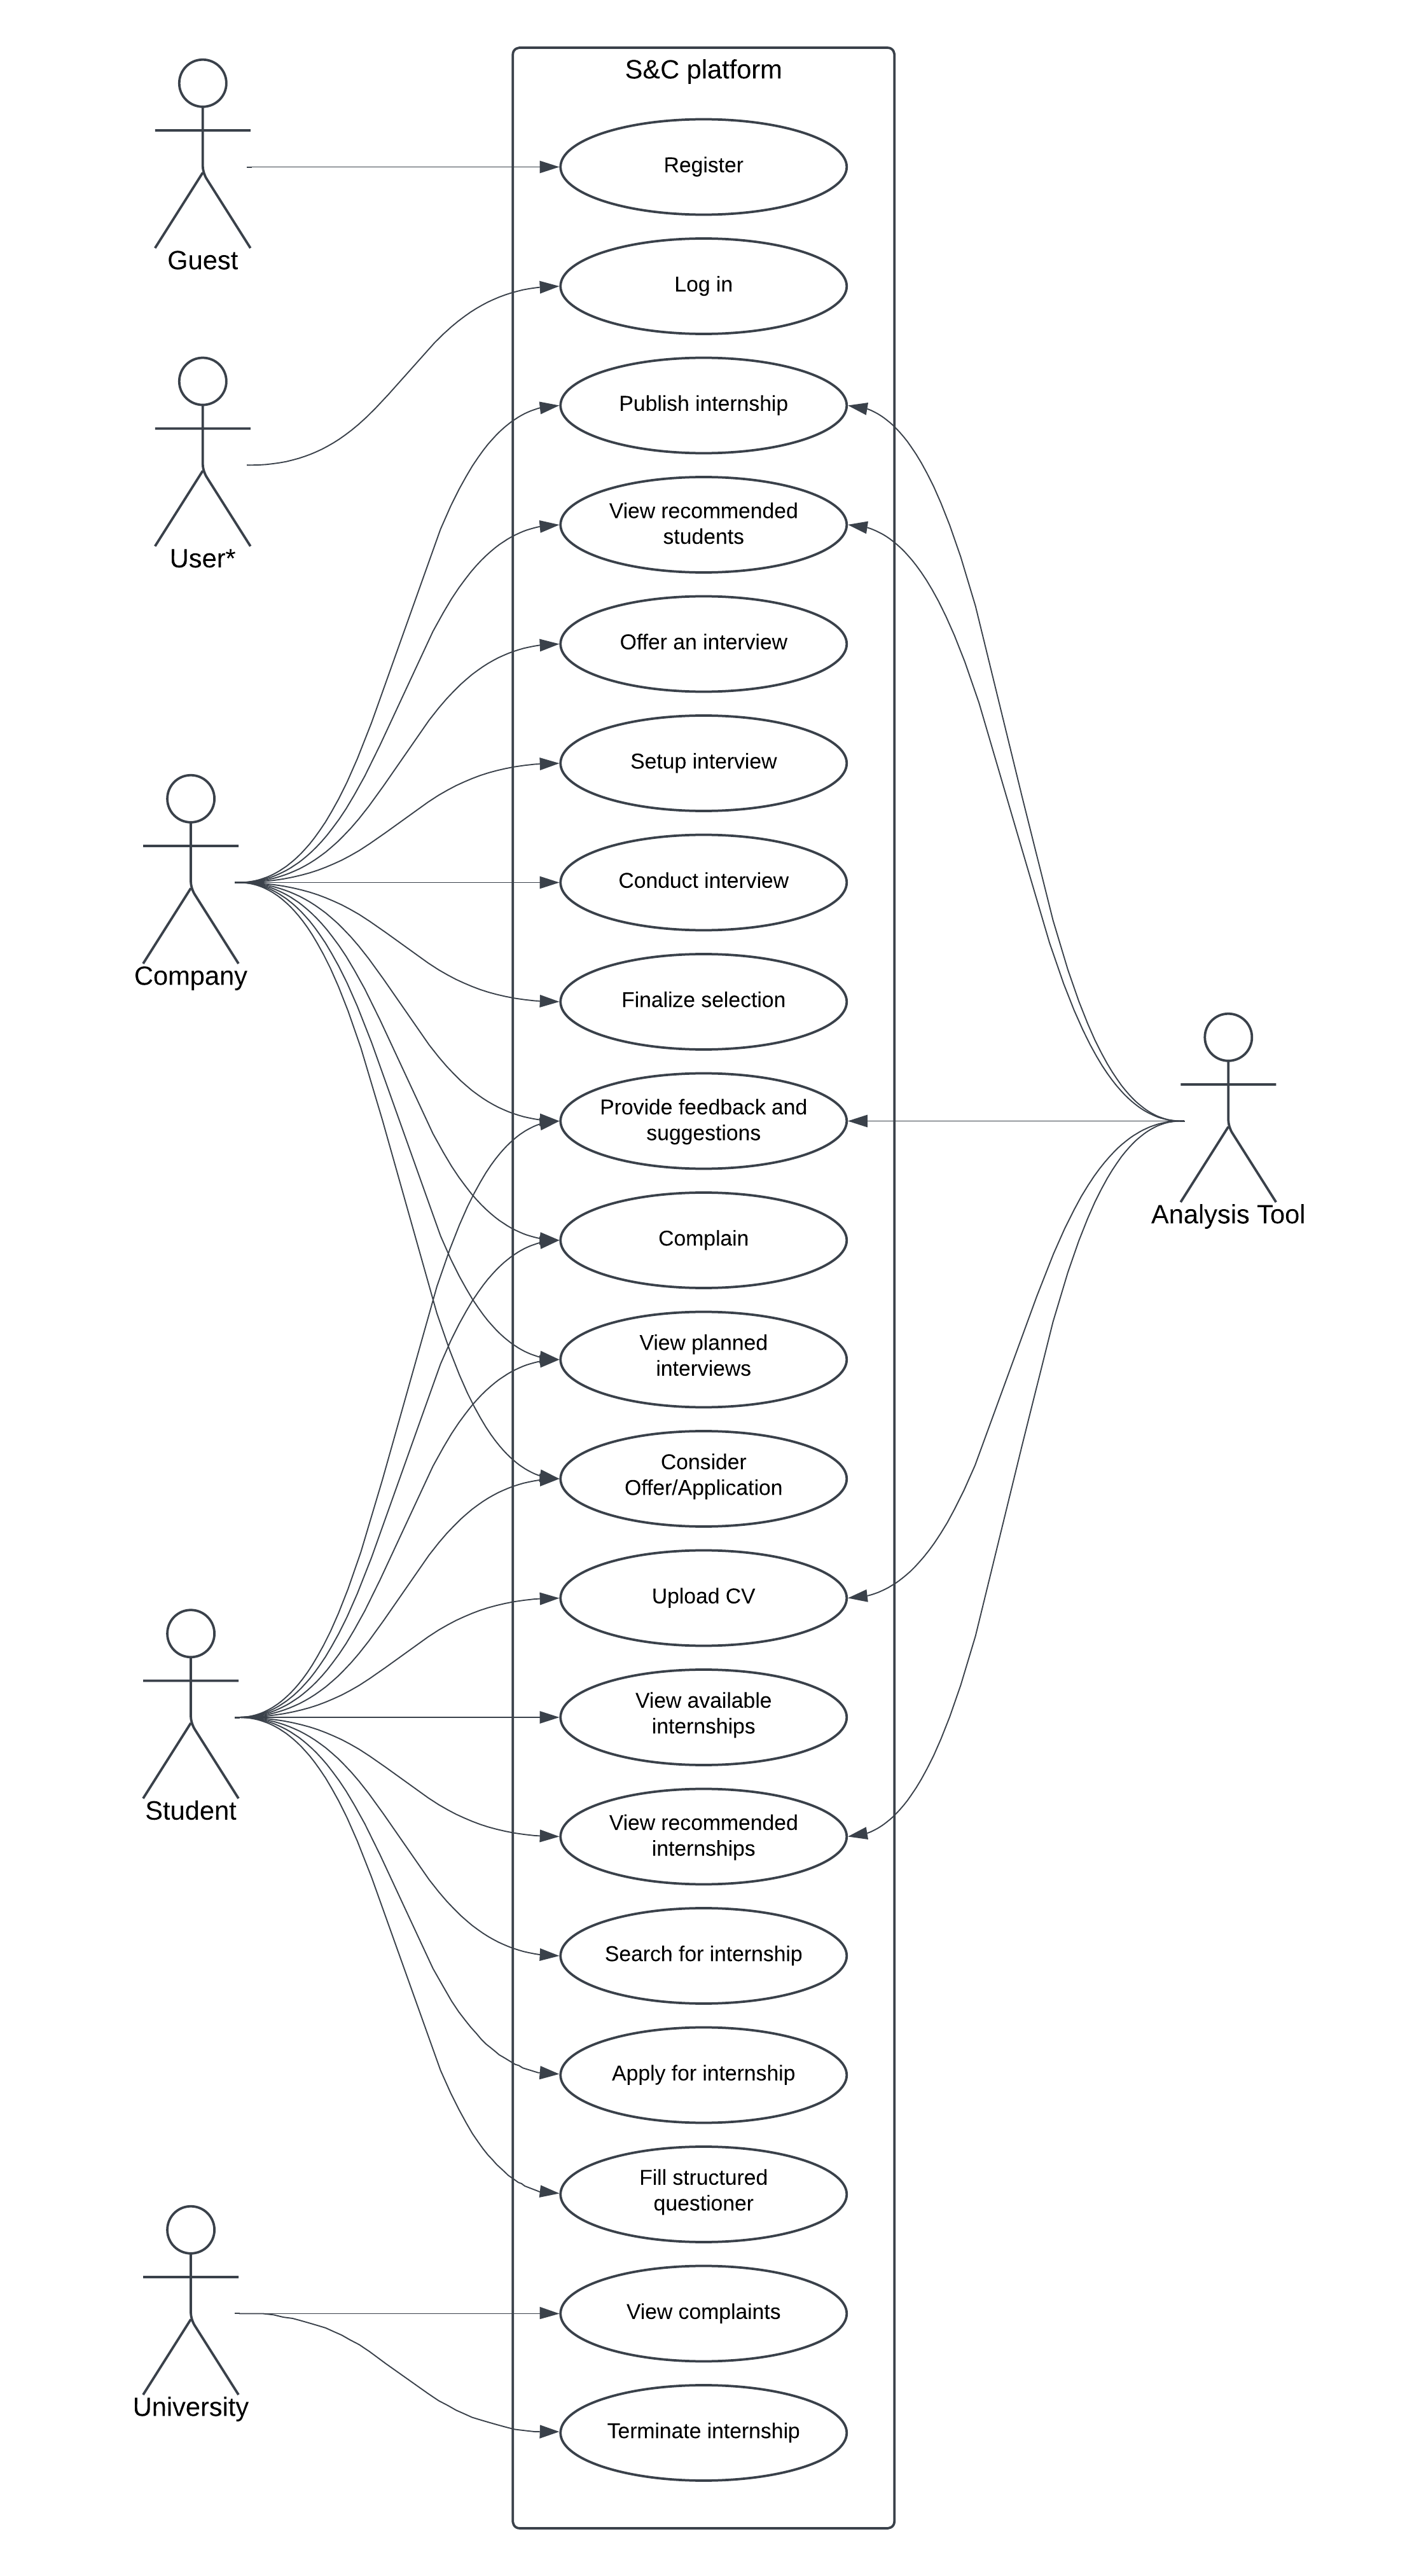
\includegraphics[width=0.8\textwidth]{Images/sd/UCD}
    \caption{Use Case Diagram}
    \label{fig:UCD}
\end{figure}

\subsection{Use cases}\label{subsec:use-cases}
In this section are depicted use cases, and for each one of them the associated sequence diagram.
\newcounter{uc}
\setcounter{uc}{1}
\newcommand{\cuc}{\theuc\stepcounter{uc}}
\begin{center}
    \begin{longtable}{|p{2.5cm}|p{10cm}|}
        \hline
        \rowcolor[HTML]{5C8A99}
        \textbf{Use Case \cuc} & \textbf{Register} \\ \hline
        \textbf{Actor} & Guest \\ \hline
        \textbf{Entry \newline conditions} & A Guest is in the landing page of S\&C and wants to register to the platform. \\ \hline
        \textbf{Event flow} &
        \begin{enumerate}
            \item The Guest clicks on the `Get Started` button.
            \item The Guest select the type of account it wants to create between student, company and university by clicking the corresponding icon.
            \item The Guest checks the `Agree to Terms and Condition` checkbox.
            \item The Guest checks the `Allow to send email notification` button.
            \item The Guest clicks on the `Get Started` button.
            \item The Guest fills the fields of the form with name, email address and password.
            \item The Guest clicks on the `Sign Up` button.
            \item The System verifies the Guest information.
            \item The System saves the Guest information.
            \item The System sends a confirmation email to the Guest.
            \item The Guest checks the provided email address inbox, and follows the link to complete the registration process.
        \end{enumerate}
        \\ \hline
        \textbf{Exit \newline condition} & The registration process is completed. \\ \hline
        \textbf{Exception} &
        \begin{itemize}
            \item If the email is already registered or of it does not exist then the System displays an error.
            \item If there are missing obligatory fields then the System displays an error.
            \item If an error occurs while saving the Guest information the System displays an error.
            \item If the selected password does not respect the defined security rules, such as minimum length and complexity, the System displays an error.
        \end{itemize}\\ \hline
    \end{longtable}
\end{center}

\begin{figure}[H]
    \centering
    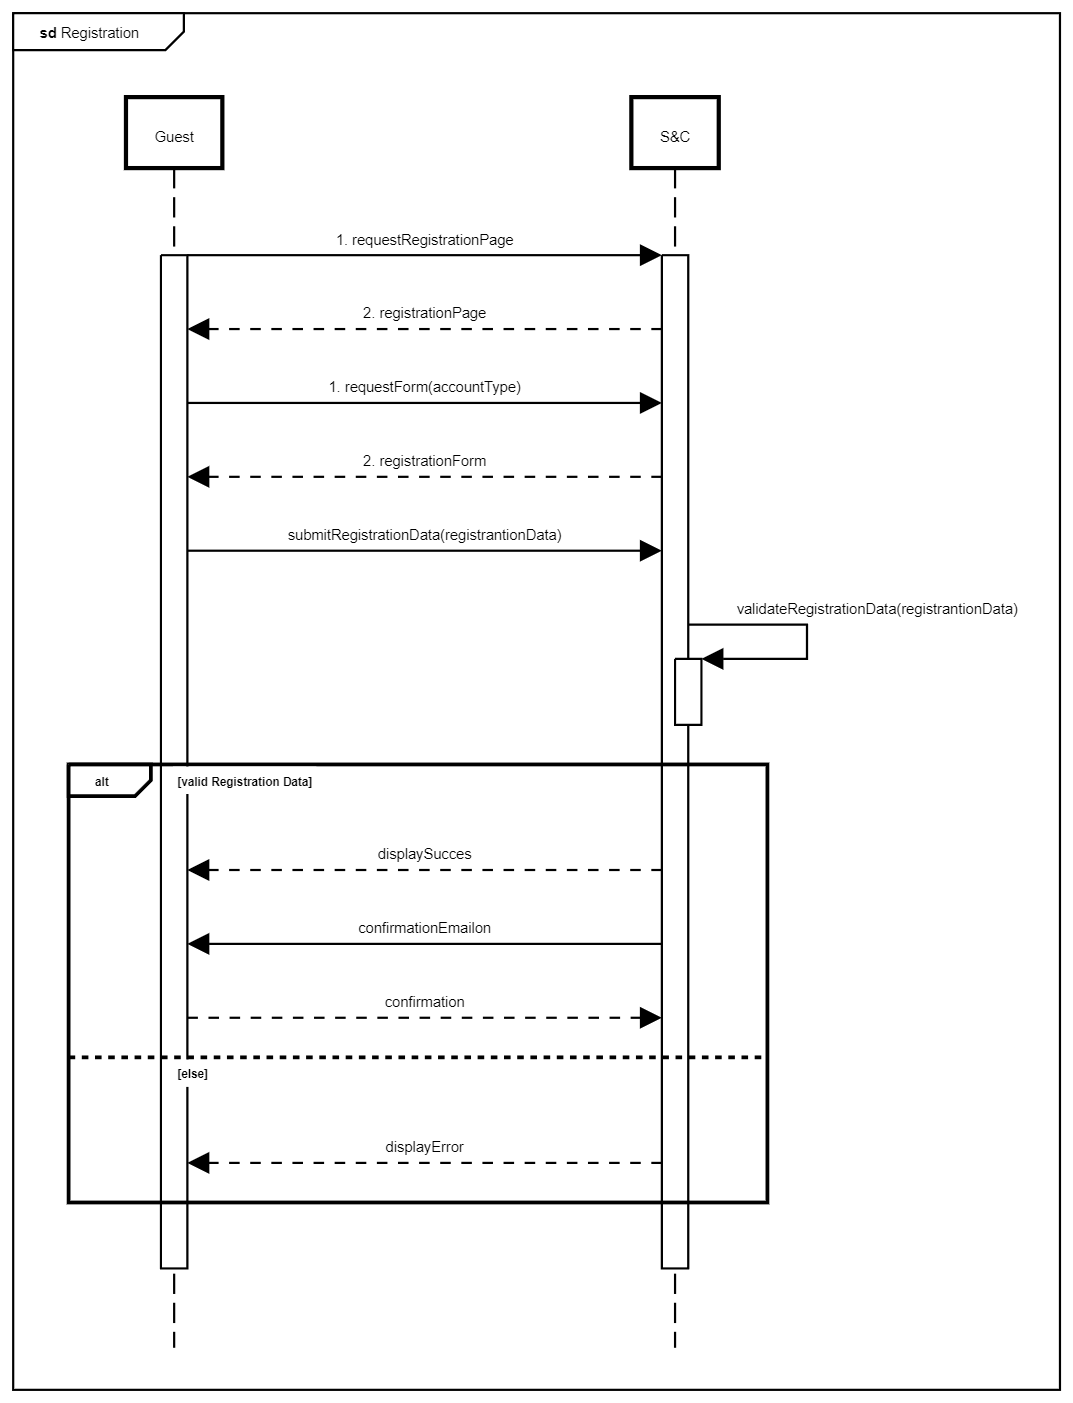
\includegraphics[width=0.8\textwidth]{Images/sd/Registration}
    \caption{Registration - Sequence Diagram}
    \label{fig:SDreg}
\end{figure}

\begin{center}
    \begin{longtable}{|p{2.5cm}|p{10cm}|}
        \hline
        \rowcolor[HTML]{5C8A99}
        \textbf{Use Case \cuc} & \textbf{Log in} \\ \hline
        \textbf{Actor} & User* \\ \hline
        \textbf{Entry \newline conditions} & The User* is in the welcome page of S\&C and wants to login in the platform. \\ \hline
        \textbf{Event flow} &
        \begin{enumerate}
            \item The User* clicks on the `Log in` button.
            \item The User* fills the fields of the form with an email address and password.
            \item The User* click on the `Log in` button.
            \item The System verifies the User information.
        \end{enumerate}
        \\ \hline
        \textbf{Exit \newline condition} & The User* is successfully logged in.\\ \hline
        \textbf{Exception} &
        \begin{itemize}
            \item If there are missing obligatory fields then the System displays an error.
            \item If an error occurs while verifying the User information the System displays an error.
            \item If the User information is not valid, that is email and/or password, the System displays an error.
        \end{itemize}
        \\ \hline
    \end{longtable}
\end{center}

\begin{figure}[H]
    \centering
    
\includegraphics[width=0.8\textwidth]{Images/sd/Login}
    \caption{Login - Sequence Diagram}
    \label{fig:SDlogin}
\end{figure}


\begin{center}
    \begin{longtable}{|p{2.5cm}|p{10cm}|}
        \hline
        \rowcolor[HTML]{5C8A99}
        \textbf{Use Case \cuc} & \textbf{Publish internship} \\ \hline
        \textbf{Actor} & Company, Analysis Tool\\ \hline
        \textbf{Entry \newline conditions} & The Company is in the publish internship section of S\&C and wants to publish a new internship on the platform. \\ \hline
        \textbf{Event flow - Main} &
        \begin{enumerate}
            \item The Company fills out the fields of the form with the position offered, the skills required, the tools, the benefits and the description of the internship.
            \item The Company clicks on the `publish` button.
            \item The System validates the information and create a new internship.
            \item The Analysis Tool elaborates the Students that would be interested in the internship.
            \item The System sends a notification to the potentially interested Students.
       \end{enumerate}
        \\ \hline
        \textbf{Event flow - Optional} &
        \begin{enumerate}
            \item The Company clicks on the suggestion button.
            \item The Analysis Tool elaborates suggestions to make the internship more appealing.
            \item The System displays the suggestions to the Company.
        \end{enumerate}
        \\ \hline
        \textbf{Exit \newline condition} & The Company successfully published a new internship on the platform and, if wanted, obtained suggestions on how to make it more appealing. \\ \hline
        \textbf{Exception} &
        \begin{itemize}
            \item If there are missing obligatory fields then the System displays an error.
            \item If an error occurs while validating the information and creating the internship the System displays an error.
            \item If an error occurs while sending a notification the System displays an error.
            \item If an error occurs while generating the interested Students the System displays an error.
            \item If an error occurs while generating suggestions the System displays an error.
            \item If an error occurs while displaying the suggestions the System displays an error.
        \end{itemize}
        \\ \hline
    \end{longtable}
\end{center}

\begin{figure}[H]
    \centering
    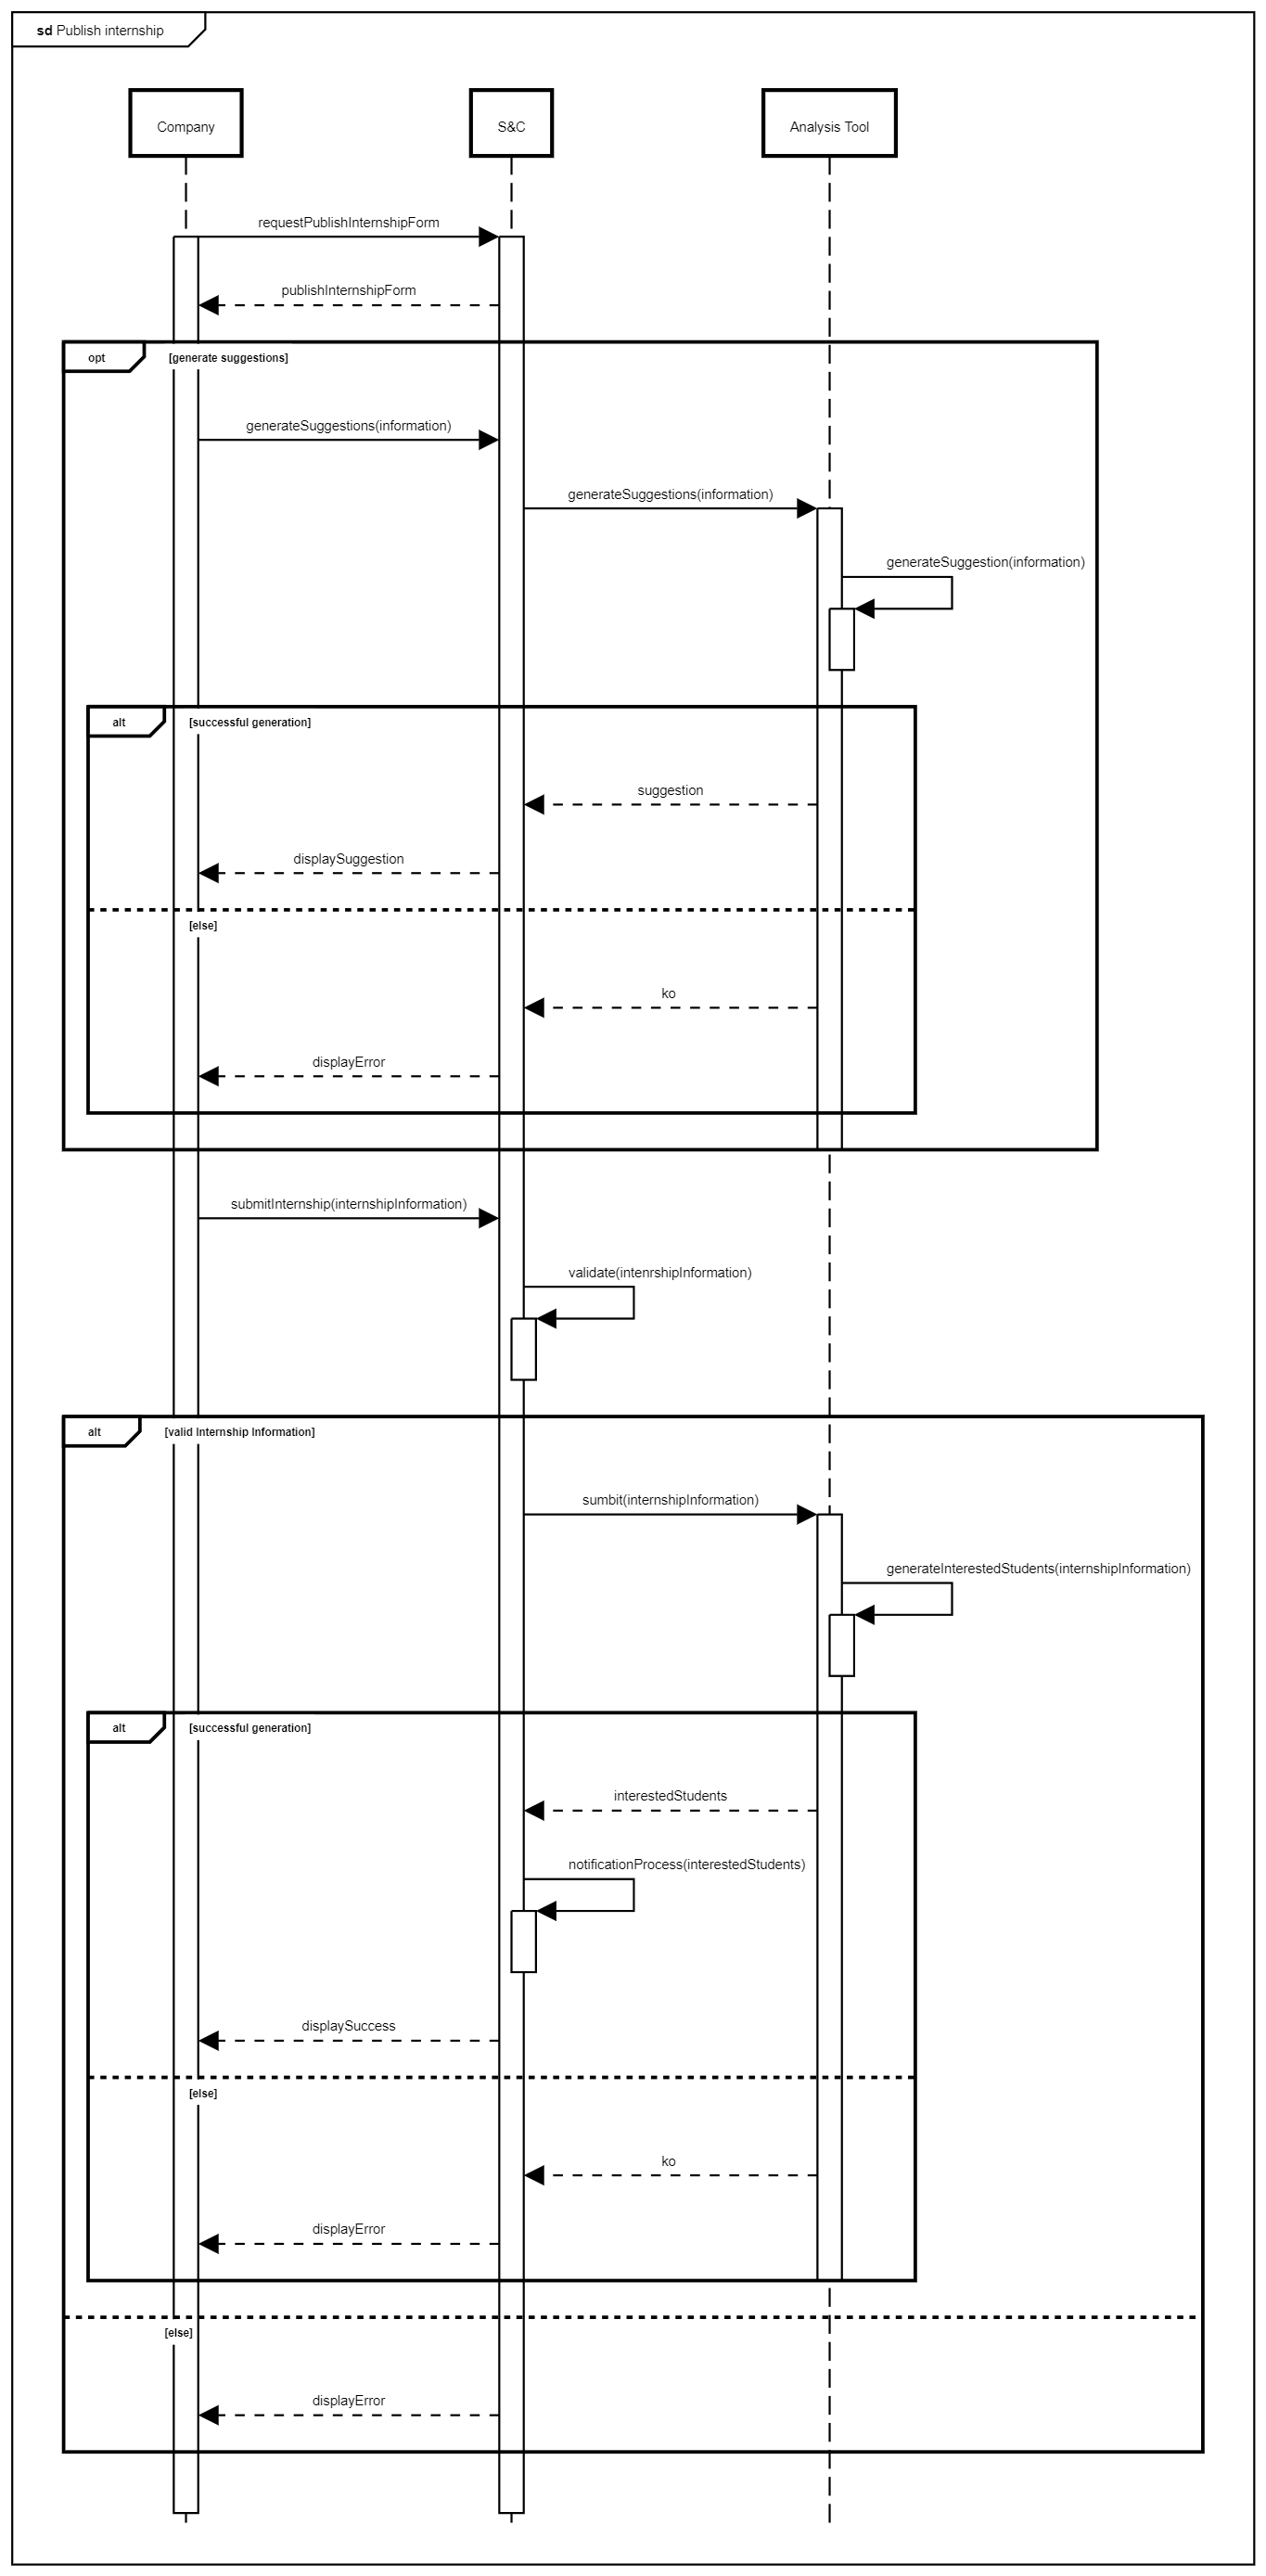
\includegraphics[width=0.8\textwidth]{Images/sd/PublishInternship}
    \caption{Publish Internship - Sequence Diagram}
    \label{fig:SDpubint}
\end{figure}


\begin{center}
    \begin{longtable}{|p{2.5cm}|p{10cm}|}
        \hline
        \rowcolor[HTML]{5C8A99}
        \textbf{Use Case \cuc} & \textbf{View recommended students} \\ \hline
        \textbf{Actor} & Company, Analysis Tool\\ \hline
        \textbf{Entry \newline conditions} & The Company is in the published internships section of S\&C and wants to see recommended Students for an internship.\\ \hline
        \textbf{Event flow - Main} &
        \begin{enumerate}
            \item The Company select the displayed internship for which it wants to see the recommended students.
            \item The Company clicks on the `recommended students` button.
            \item The Analysis Tool compute the recommended students based on internship information.
            \item The System redirects the Company to the view recommended section.
        \end{enumerate}
        \\ \hline
        \textbf{Event flow - Optional} &
        \begin{enumerate}
            \item The Company select a Student from the list to view its details.
            \item The Company filter the recommended Students by writing in the appropriate search box.
        \end{enumerate}
        \\ \hline
        \textbf{Exit \newline condition} & The Company successfully views the recommended Students, and if wanted, view the details of some of the them. \\ \hline
        \textbf{Exception} &
        \begin{itemize}
            \item If an error occurs while redirecting the Company the System displays an error.
            \item If the are no recommended Students the System displays an error.
            \item If an error occurs while showing the details of a Student the System displays an error.
            \item If an error occurs while filtering recommended Students the System displays an error.
            \item If an error occurs while the Analysis tool compute the recommendations the System displays an error.
        \end{itemize}
        \\ \hline
    \end{longtable}
\end{center}

\begin{figure}[H]
    \centering
    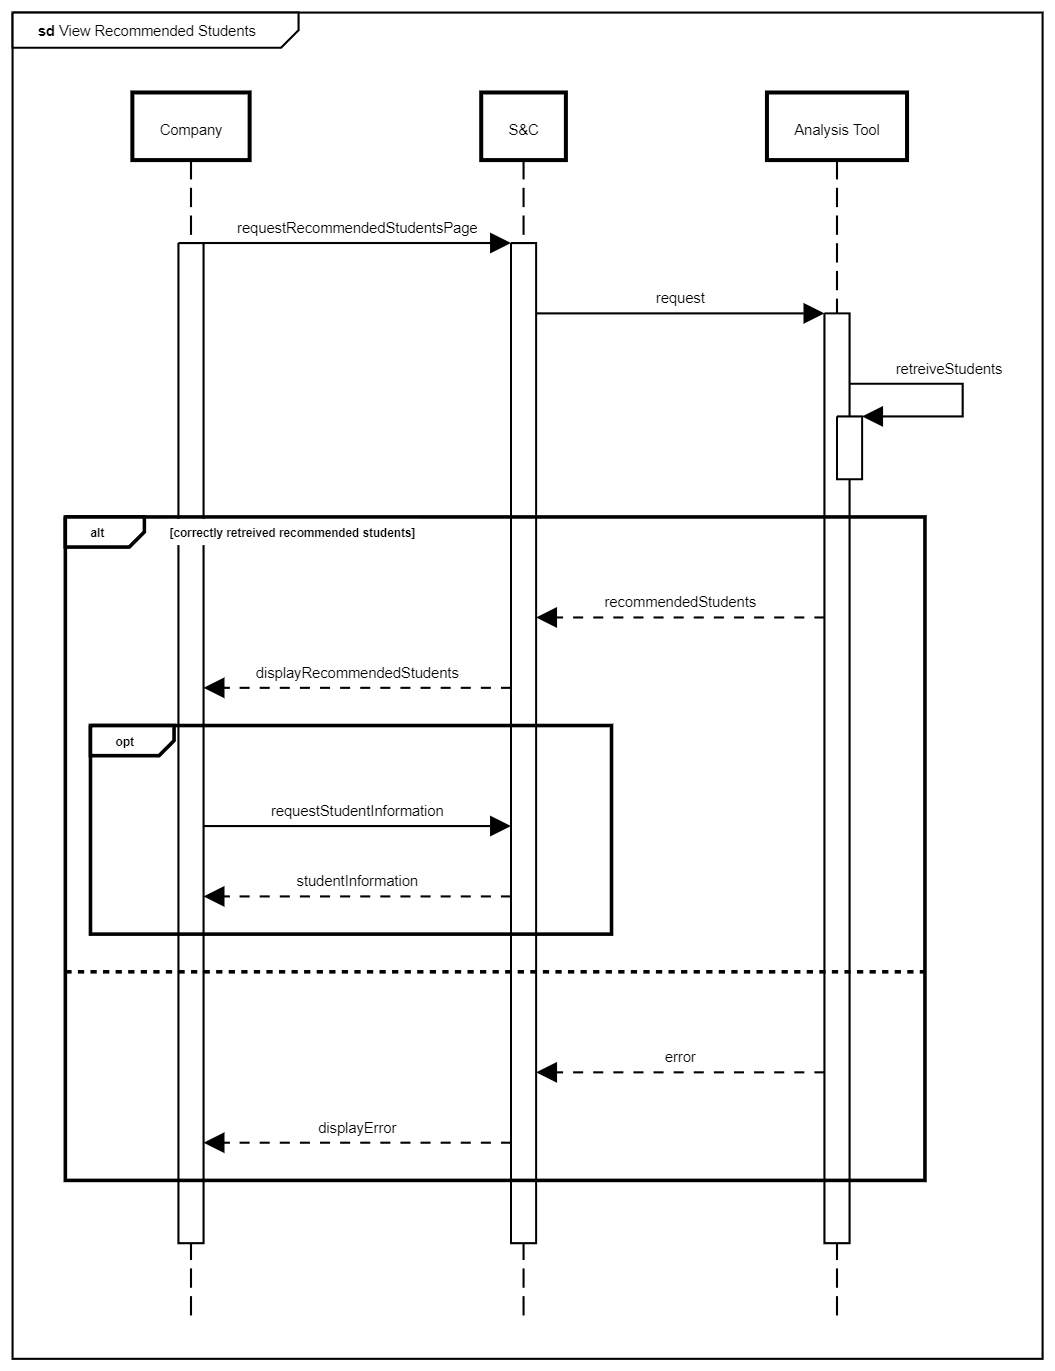
\includegraphics[width=0.8\textwidth]{Images/sd/ViewRecommendedStudents}
    \caption{View recommended students - Sequence Diagram}
    \label{fig:SDviewrecstud}
\end{figure}


\begin{center}
    \begin{longtable}{|p{2.5cm}|p{10cm}|}
        \hline
        \rowcolor[HTML]{5C8A99}
        \textbf{Use Case \cuc} & \textbf{Offer an interview} \\ \hline
        \textbf{Actor} & Company \\ \hline
        \textbf{Entry \newline conditions} & The Company is in the recommended students list for an internship and wants to send an interview proposal. \\ \hline
        \textbf{Event flow} &
        \begin{enumerate}
            \item The Company navigate to the detail page of the selected Student.
            \item The Company click on the `send offer` button.
            \item The System sends a notification to the Student with the interview offer.
        \end{enumerate}
        \\ \hline
        \textbf{Exit \newline condition} & The Company successfully sent an interview offer. \\ \hline
        \textbf{Exception} &
        \begin{itemize}
            \item If an error occurs while validating the information the System displays an error.
            \item If an error occurs while sending a notification the System displays an error.
        \end{itemize}
        \\ \hline
    \end{longtable}
\end{center}

\begin{figure}[H]
    \centering
    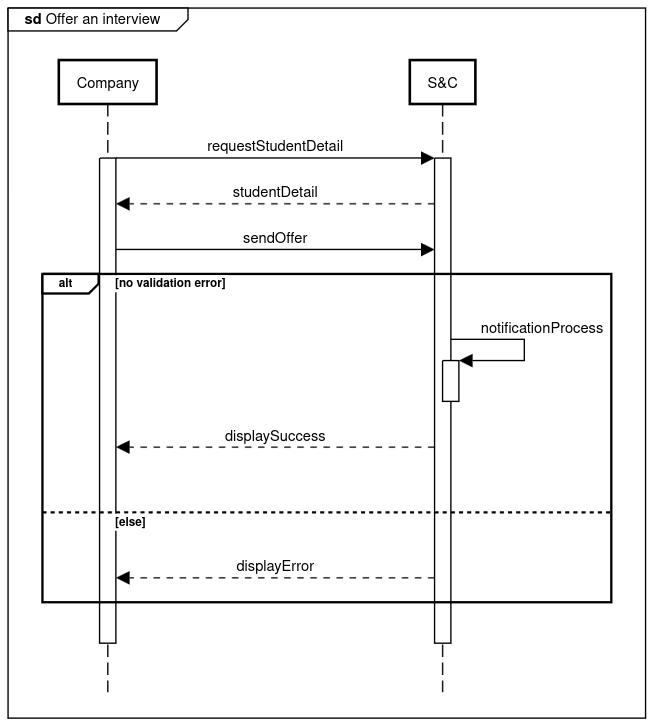
\includegraphics[width=0.8\textwidth]{Images/sd/OfferInterview}
    \caption{Offer interview - Sequence Diagram}
    \label{fig:SDofferint}
\end{figure}

\begin{center}
    \begin{longtable}{|p{2.5cm}|p{10cm}|}
        \hline
        \rowcolor[HTML]{5C8A99}
        \textbf{Use Case \cuc} & \textbf{Setup interview} \\ \hline
         \textbf{Actor} & Company \\ \hline
        \textbf{Entry \newline conditions} & The Company is in the setup interview section of S\&C and wants to set up a new interview on the platform. \\ \hline
        \textbf{Event flow} &
        \begin{enumerate}
            \item The Company fills the fields with the date, time, candidate and additional notes of the new interview.
            \item The Company adds the questions for the structured questioner by clicking on the `plus` button.
            \item The Company click on the `Setup` button.
            \item The System validates the information and create a new interview.
            \item The System sends a notification to the selected candidate for the interview.
        \end{enumerate}
        \\ \hline
        \textbf{Exit \newline condition} & The Company successfully set up a new interview on the platform. \\ \hline
        \textbf{Exception} &
        \begin{itemize}
            \item If there are missing obligatory fields then the System displays an error.
            \item If an error occurs while validating the information and creating the interview the System displays an error.
            \item If an error occurs while sending a notification the System displays an error.
        \end{itemize}
        \\ \hline
    \end{longtable}
\end{center}

\begin{figure}[H]
    \centering
    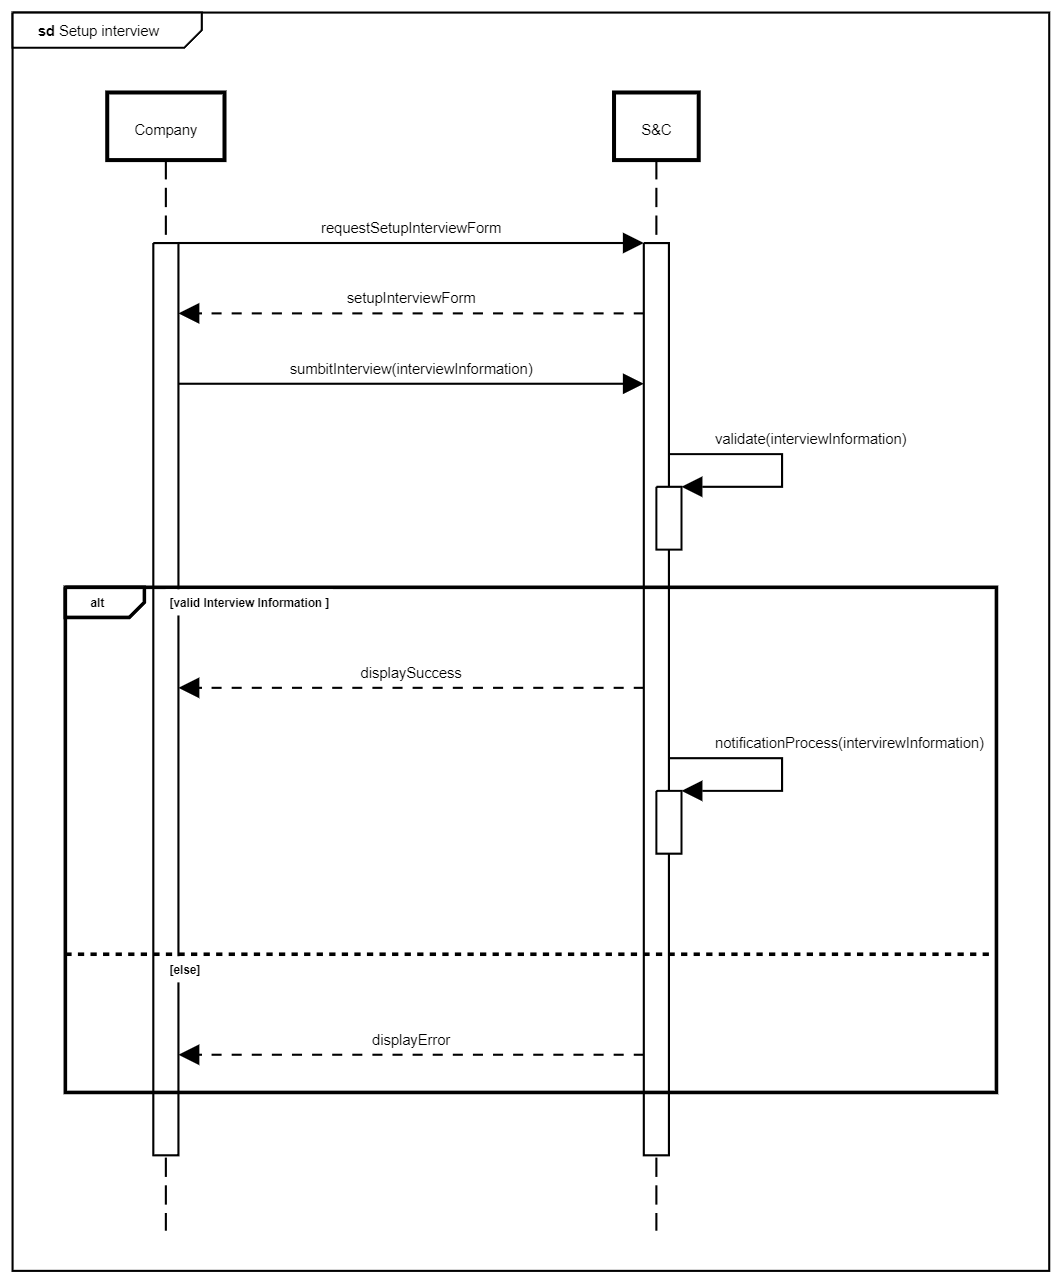
\includegraphics[width=0.8\textwidth]{Images/sd/SetupInterview}
    \caption{Setup interview - Sequence Diagram}
    \label{fig:SDsetupint}
\end{figure}

\begin{center}
    \begin{longtable}{|p{2.5cm}|p{10cm}|}
        \hline
        \rowcolor[HTML]{5C8A99}
        \textbf{Use Case \cuc} & \textbf{Conduct interview} \\ \hline
        \textbf{Actor} & Company \\ \hline
        \textbf{Entry \newline conditions} & The Company is in the view planned interview section of S\&C and wants to evaluate a student during an interview. \\ \hline
        \textbf{Event flow - Main} &
        \begin{enumerate}
            \item The Company clicks on the 'Evaluate' button.
            \item The Company gets redirected to the Conduct Interview page.
            \item The Company fill the form with a technical score, personal score and a company fit score.
            \item The Company clicks the `confirm` button.
            \item The System validates the information and saves the result of the interview.
        \end{enumerate}
        \\ \hline
        \textbf{Event flow - Optional} &
        \begin{enumerate}
            \item The Company complete the additional notes field for during the interview.
        \end{enumerate}
        \\ \hline
        \textbf{Exit \newline condition} & The Company successfully finished the interview and the result is saved on the platform. \\ \hline
        \textbf{Exception} &
        \begin{itemize}
            \item If there are missing obligatory fields then the System displays an error.
            \item If an error occurs while validating the information and saving the interview result the System displays an error.
        \end{itemize}
        \\ \hline
    \end{longtable}
\end{center}

\begin{figure}[H]
    \centering
    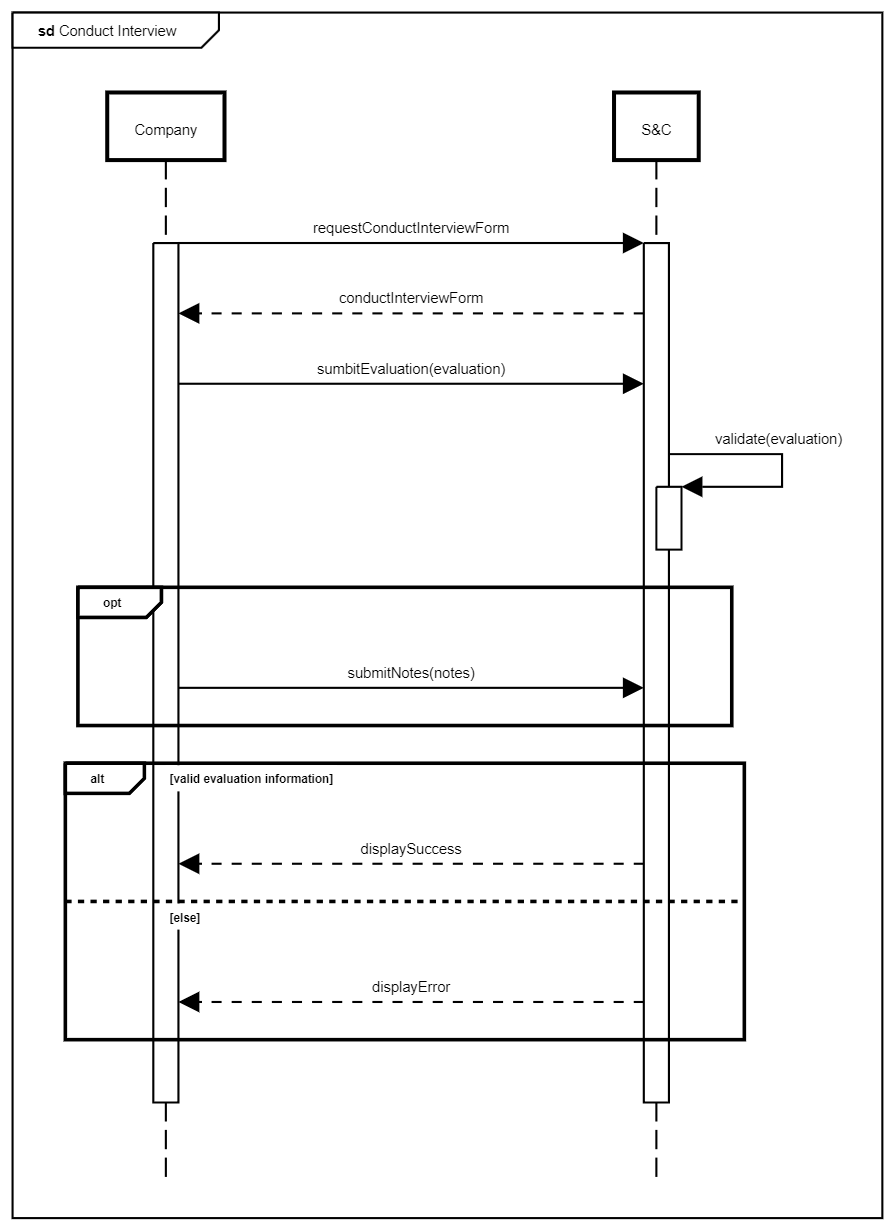
\includegraphics[width=0.8\textwidth]{Images/sd/ConductInterview}
    \caption{Conduct interview - Sequence Diagram}
    \label{fig:SDconduct}
\end{figure}


\begin{center}
    \begin{longtable}{|p{2.5cm}|p{10cm}|}
        \hline
        \rowcolor[HTML]{5C8A99}
        \textbf{Use Case \cuc} & \textbf{Finalize selection} \\ \hline
        \textbf{Actor} & Company \\ \hline
        \textbf{Entry \newline conditions} & The Company selected an interview in the view published internships section of the S\&C platform and wants to finalize the selection of candidates. \\ \hline
        \textbf{Event flow} &
        \begin{enumerate}
            \item The Company clicks on the 'Finalize' button.
            \item The Company gets redirected to the finalize page.
            \item The Company select among the possible candidates sorted by evaluation score.
            \item The Company views the responses to the questions filled in the structured questioner, as well as the evaluation information for that candidate .
            \item The Company confirm the choice by clicking the `confirm` button.
            \item The System notifies the selected candidate and closes the internship position temporarily.
        \end{enumerate}
        \\ \hline
        \textbf{Exit \newline condition} & The Company successfully finalized the selection. \\ \hline
        \textbf{Exception} &
        \begin{itemize}
            \item If an error occurs while the Company select the candidate System displays an error.
            \item If an error occurs while sending a notification the System displays an error.
            \item If an error occurs while closing the internship position temporarily the System displays an error.
        \end{itemize}
        \\ \hline
    \end{longtable}
\end{center}

\begin{figure}[H]
    \centering
    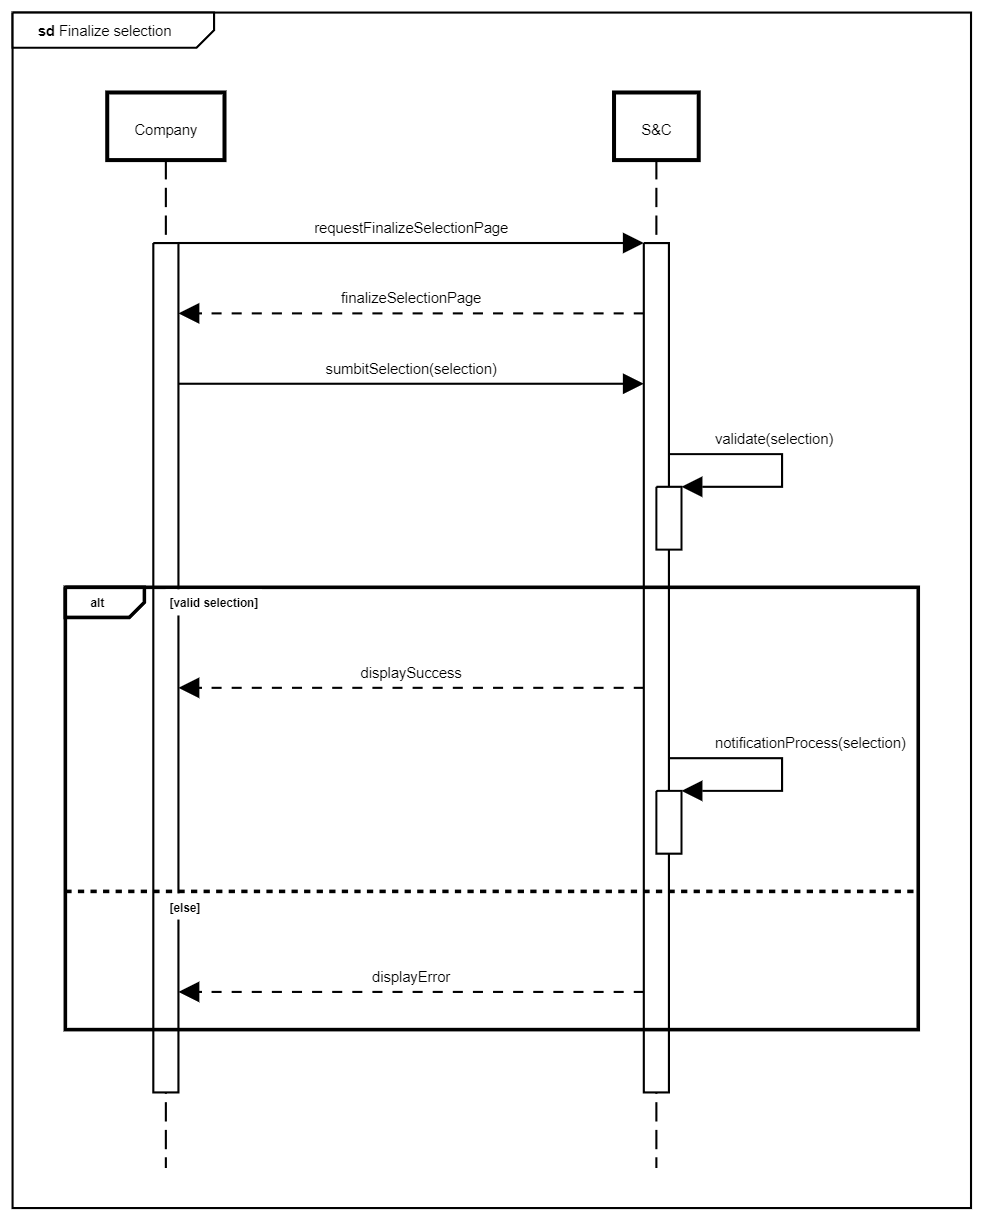
\includegraphics[width=0.8\textwidth]{Images/sd/FinalizeSelection}
    \caption{Finalize selection - Sequence Diagram}
    \label{fig:SDfinalize}
\end{figure}


\begin{center}
    \begin{longtable}{|p{2.5cm}|p{10cm}|}
        \hline
        \rowcolor[HTML]{5C8A99}
        \textbf{Use Case \cuc} & \textbf{Provide feedback and suggestions} \\ \hline
        \textbf{Actor} & User, Analysis Tool \\ \hline
        \textbf{Entry \newline conditions} & The User is in the provide feedback form of the S\&C platform and wants to provide feedback and suggestions.\\ \hline
        \textbf{Event flow} &
        \begin{enumerate}
            \item The User fills the form with feedback and suggestions.
            \item The User gives a rating out of five stars.
            \item The User clicks the `submit` button.
            \item The System feeds the information to the Analysis Tool.
        \end{enumerate}
        \\ \hline
        \textbf{Exit \newline condition} & The User successfully provided feedback and suggestions\\ \hline
        \textbf{Exception} &
        \begin{itemize}
            \item If there are missing obligatory fields then the System displays an error.
            \item If an error occurs while feeding the Analysis Tool the System displays an error.
        \end{itemize}
        \\ \hline
    \end{longtable}
\end{center}

\begin{figure}[H]
    \centering
    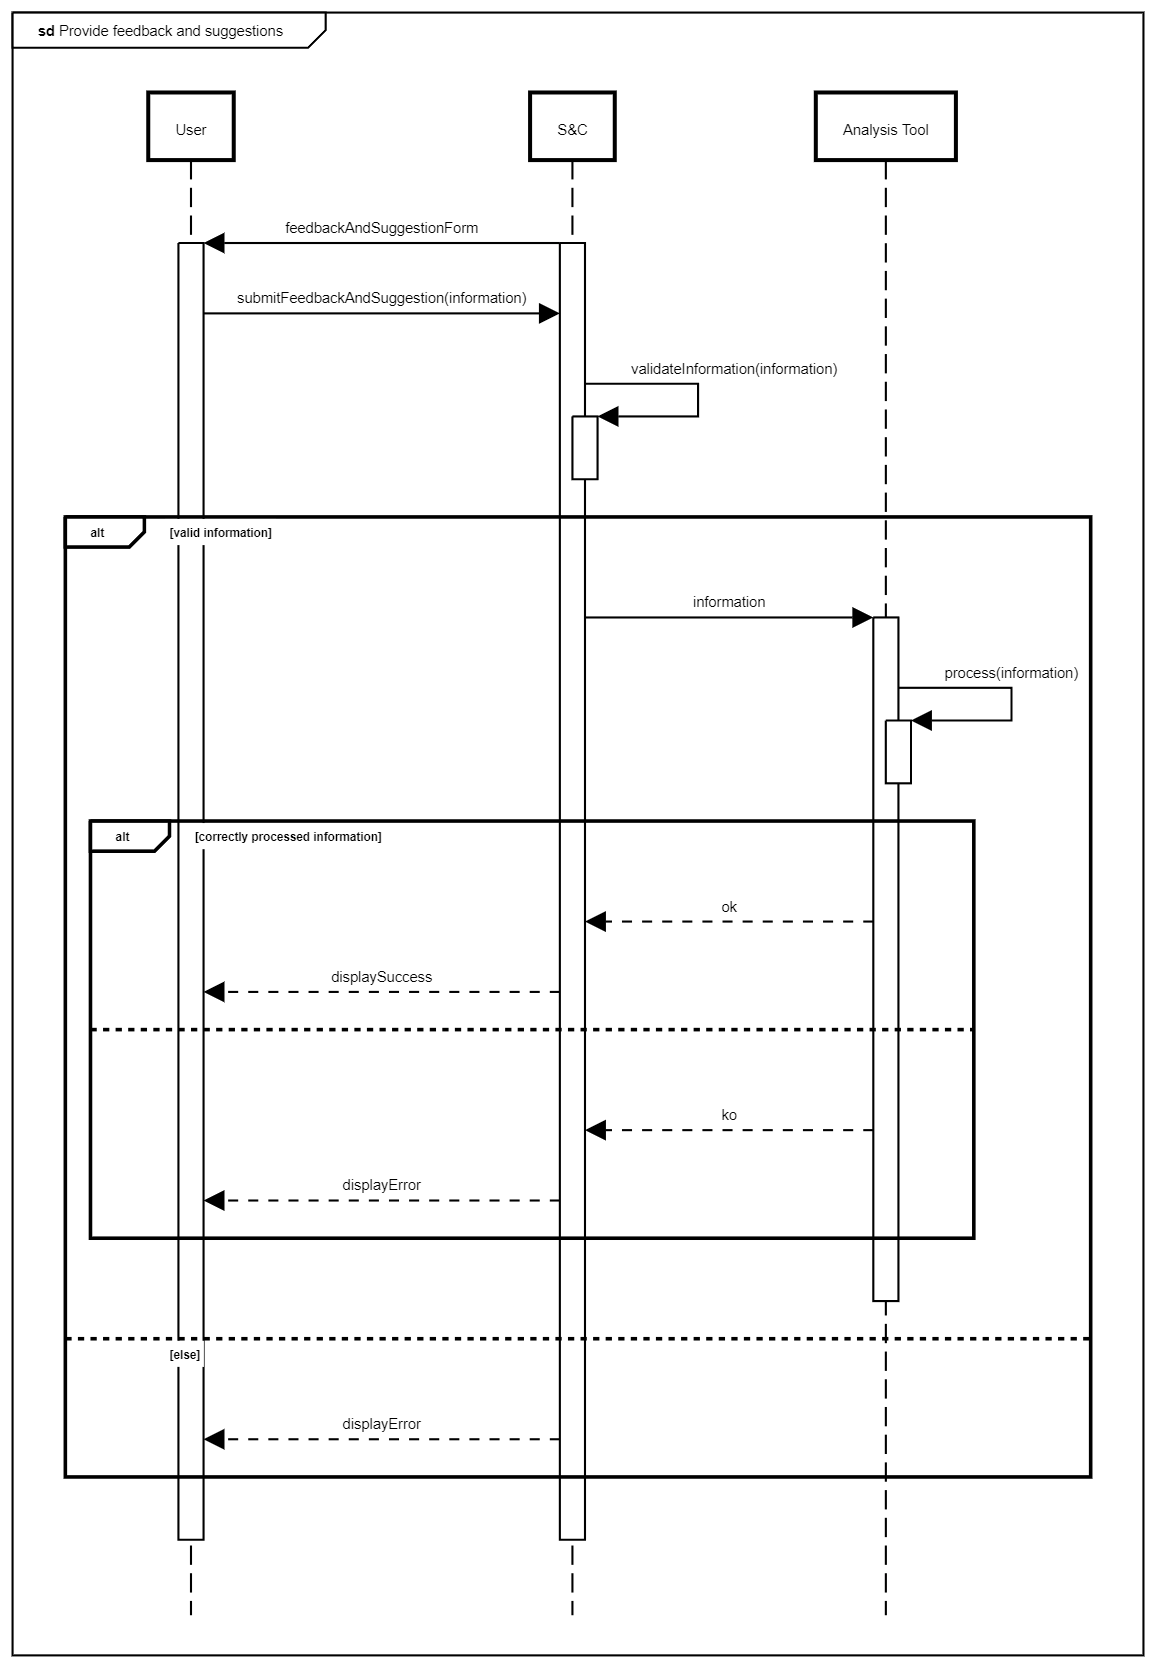
\includegraphics[width=0.8\textwidth]{Images/sd/FeedbackAndSuggestions}
    \caption{Provide feedback and suggestions - Sequence Diagram}
    \label{fig:SDfeedandsug}
\end{figure}

\begin{center}
    \begin{longtable}{|p{2.5cm}|p{10cm}|}
        \hline
        \rowcolor[HTML]{5C8A99}
        \textbf{Use Case \cuc} & \textbf{Complain} \\ \hline
        \textbf{Actor} & User \\ \hline
        \textbf{Entry \newline conditions} & The User is in the complain section of S\&C and wants to send a complaint to the university responsible for overseeing an internship\\ \hline
        \textbf{Event flow} &
        \begin{enumerate}
            \item The User select the internship for which he wants to send a complain.
            \item The User fills in the description of the complaint.
            \item The User click the `publish` button.
            \item The System validates the information and creates a new complaint.
            \item The System send a notification to the University overseeing the internship.
        \end{enumerate}
        \\ \hline
        \textbf{Exit \newline condition} & The User successfully sent the complain. \\ \hline
        \textbf{Exception} &
        \begin{itemize}
            \item If there are missing obligatory fields then the System displays an error.
            \item If an error occurs while the User select the internship the System displays an error.
            \item If an error occurs while sending a notification the System displays an error.
        \end{itemize}
        \\ \hline
    \end{longtable}
\end{center}

\begin{figure}[H]
    \centering
    
\includegraphics[width=0.8\textwidth]{Images/sd/Complain}
    \caption{Complain - Sequence Diagram}
    \label{fig:SDcomplain}
\end{figure}

\begin{center}
    \begin{longtable}{|p{2.5cm}|p{10cm}|}
        \hline
        \rowcolor[HTML]{5C8A99}
        \textbf{Use Case \cuc} & \textbf{View planned interviews} \\ \hline
        \textbf{Actor} & User \\ \hline
        \textbf{Entry \newline conditions} & The User is in the main section of S\&C and wants to view planned interviews.\\ \hline
        \textbf{Event flow - Main} &
        \begin{enumerate}
            \item The User clicks on the `view planned interviews' section.
            \item The System displays the list of planned interviews.
        \end{enumerate}
        \\ \hline
        \textbf{Event flow - Optional} &
        \begin{enumerate}
            \item The User filter by name the planned interviews by writing in the appropriate search box.
            \item The User filter by date the planned interviews by selecting the date in the drop down list.
            \item The User clicks on the desired planned interview and the System shows some details such as date, time and notes of that interview.
        \end{enumerate}
        \\ \hline
        \textbf{Exit \newline condition} & The User successfully viewed the planned interviews, and if wanted, filtered and visualized some details of some of them. \\ \hline
        \textbf{Exception} &
        \begin{itemize}
            \item If the are no planned interviews the System displays a `no planned interviews` message.
            \item If an error occurs while showing the the details of an interview the System displays an error.
            \item If an error occurs while filtering planned interviews the System displays an error.
        \end{itemize}
        \\ \hline
    \end{longtable}
\end{center}

\begin{figure}[H]
    \centering
    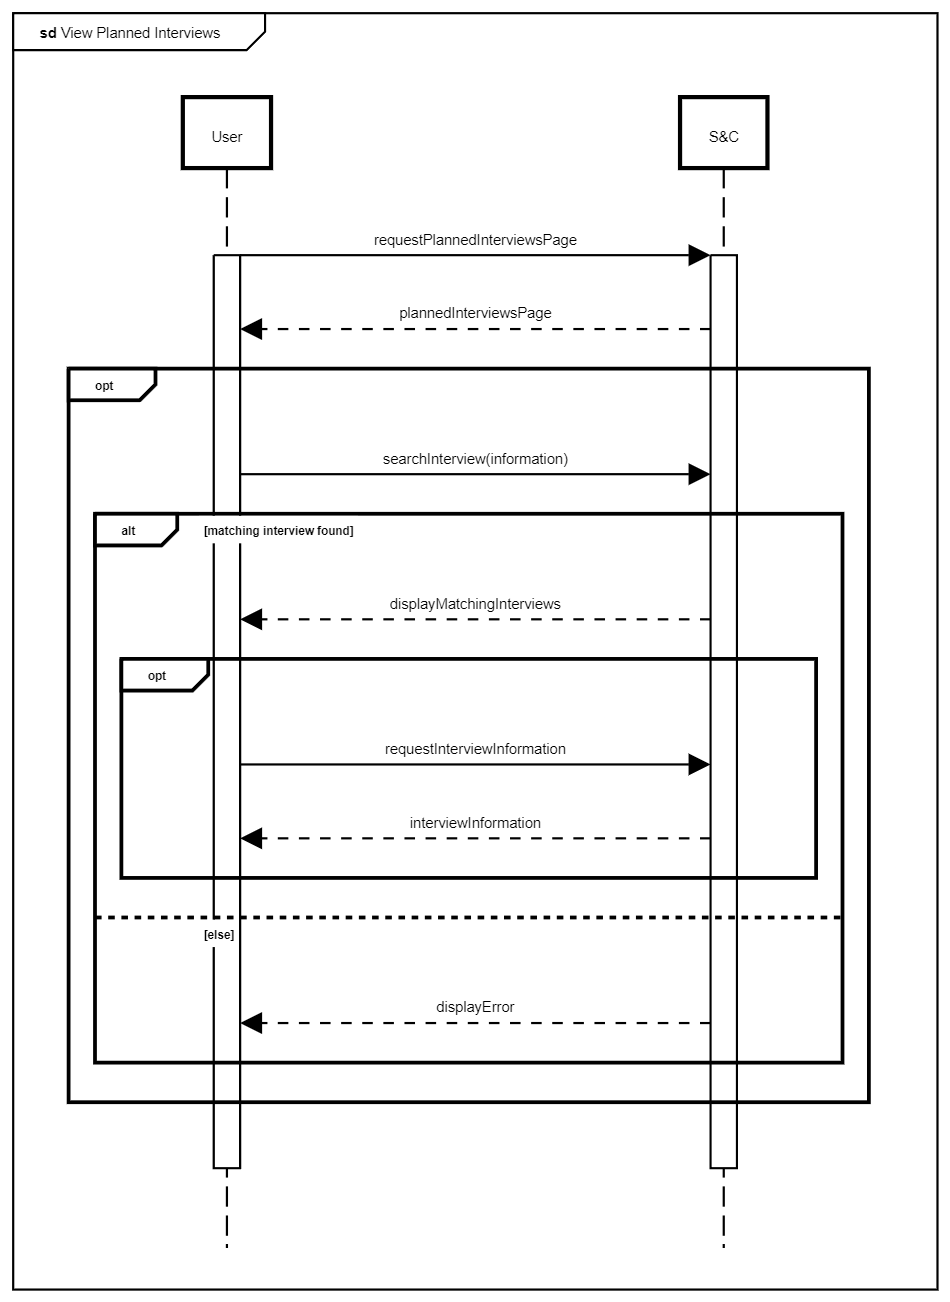
\includegraphics[width=0.8\textwidth]{Images/sd/ViewPlannedInterviews}
    \caption{View planned interviews - Sequence Diagram}
    \label{fig:SDviewplannedinterviews}
\end{figure}

\begin{center}
    \begin{longtable}{|p{2.5cm}|p{10cm}|}
        \hline
        \rowcolor[HTML]{5C8A99}
        \textbf{Use Case \cuc} & \textbf{Consider offer/application} \\ \hline
        \textbf{Actor} &  User \\ \hline
        \textbf{Entry \newline conditions} & The User is in the notification center of the S\&C platform and wants to accept or reject an offer/application. \\ \hline
        \textbf{Event flow} &
        \begin{enumerate}
            \item The User select the offer/application from the displayed notification.
            \item The User express the choice to reject or accept.
            \item The System sends a notification to the counterpart of the offer/application.
        \end{enumerate}
        \\ \hline
        \textbf{Exit \newline condition} & The User successfully accepted or rejected an offer/application. \\ \hline
        \textbf{Exception} &
        \begin{itemize}
            \item If an error occurs while validating the information the System displays an error.
            \item If an error occurs while sending a notification the System displays an error.
        \end{itemize}
        \\ \hline
    \end{longtable}
\end{center}

\begin{figure}[H]
    \centering
    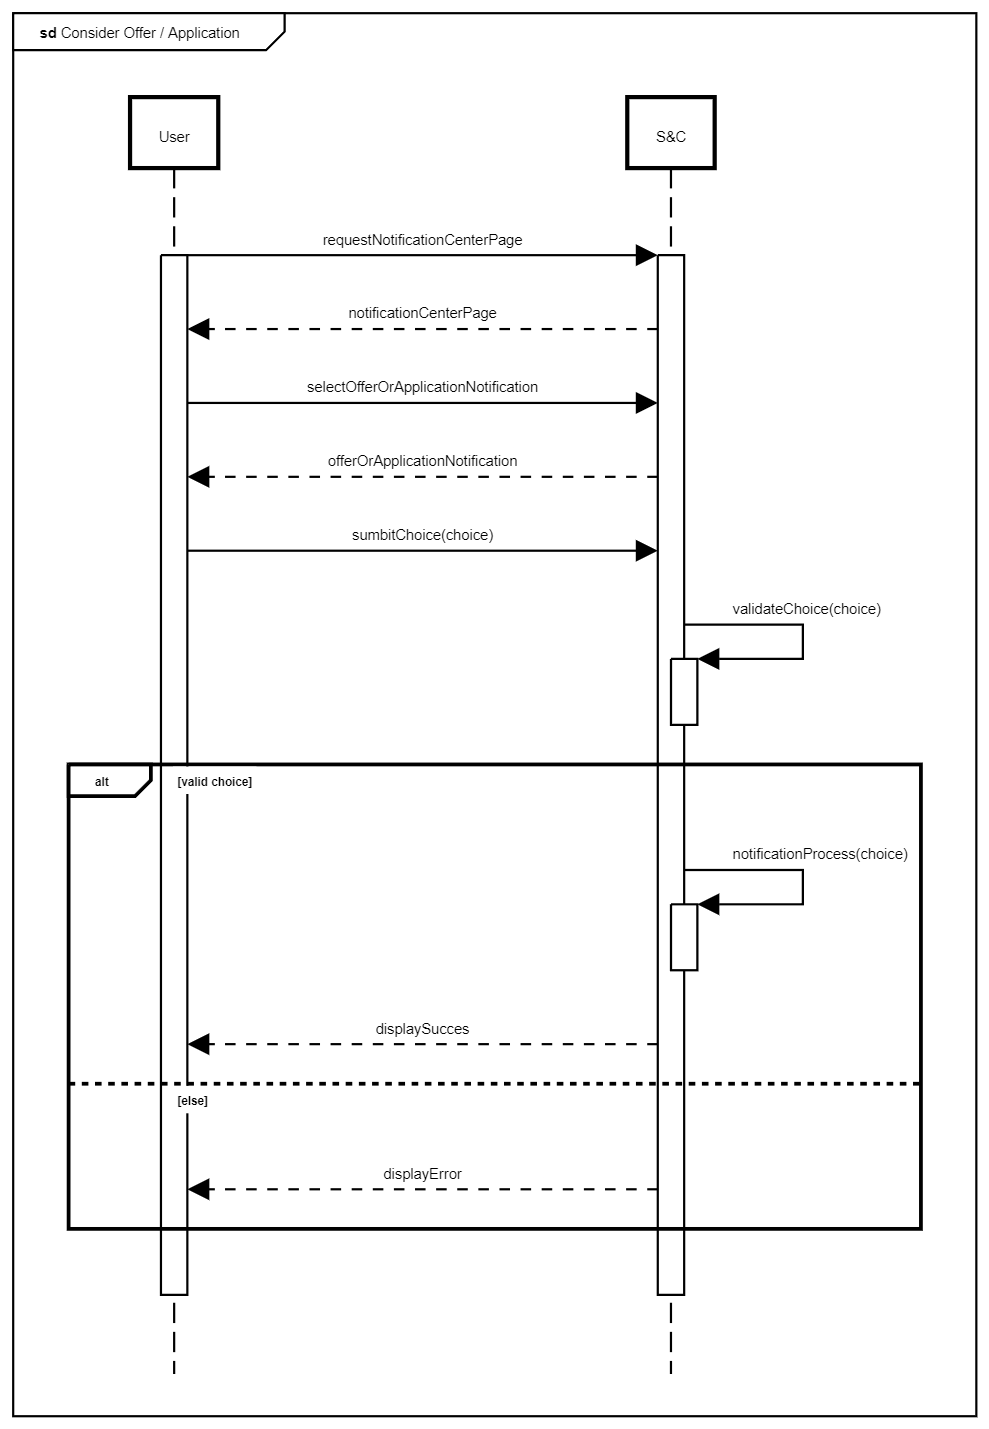
\includegraphics[width=0.8\textwidth]{Images/sd/ConsiderOfferApplication}
    \caption{Consider offer/application - Sequence Diagram}
    \label{fig:SDconsiderofferapplication}
\end{figure}

\begin{center}
    \begin{longtable}{|p{2.5cm}|p{10cm}|}
        \hline
        \rowcolor[HTML]{5C8A99}
        \textbf{Use Case \cuc} & \textbf{Upload CV} \\ \hline
        \textbf{Actor} & Student, Analysis Tool \\ \hline
        \textbf{Entry \newline conditions} & The Student is in the modify personal data section of S\&C and wants to upload the CV.\\ \hline
        \textbf{Event flow - Main} &
        \begin{enumerate}
            \item The Student clicks on the upload icon and uploads the CV.
            \item The Student clicks on the `Upload` button.
            \item The System validates the information and updates the CV of the Student.
            \item The Analysis Tool elaborates suggestions to make the CV more appealing.
            \item The System displays the suggestions to the Student.
            \item The Analysis Tool elaborates the Companies that would be interested in the Student.
            \item The System sends a notification to the potentially interested Companies.
        \end{enumerate}
        \\ \hline
        \textbf{Exit \newline condition} & The Student successfully updated the CV and obtained suggestions on how to make it more appealing. \\ \hline
        \textbf{Exception} &
        \begin{itemize}
            \item If there are missing obligatory fields then the System displays an error.
            \item If an error occurs while the Student select the CV to upload the System displays an error.
            \item If an error occurs while validating and updating the CV of the Student the System displays an error.
            \item If an error occurs while sending a notification the System displays an error.
            \item If an error occurs while generating the interested Companies the System displays an error.
            \item If an error occurs while generating suggestions the System displays an error.
            \item If an error occurs while displaying the suggestions the System displays an error.
        \end{itemize}
        \\ \hline
    \end{longtable}
\end{center}

\begin{figure}[H]
    \centering
    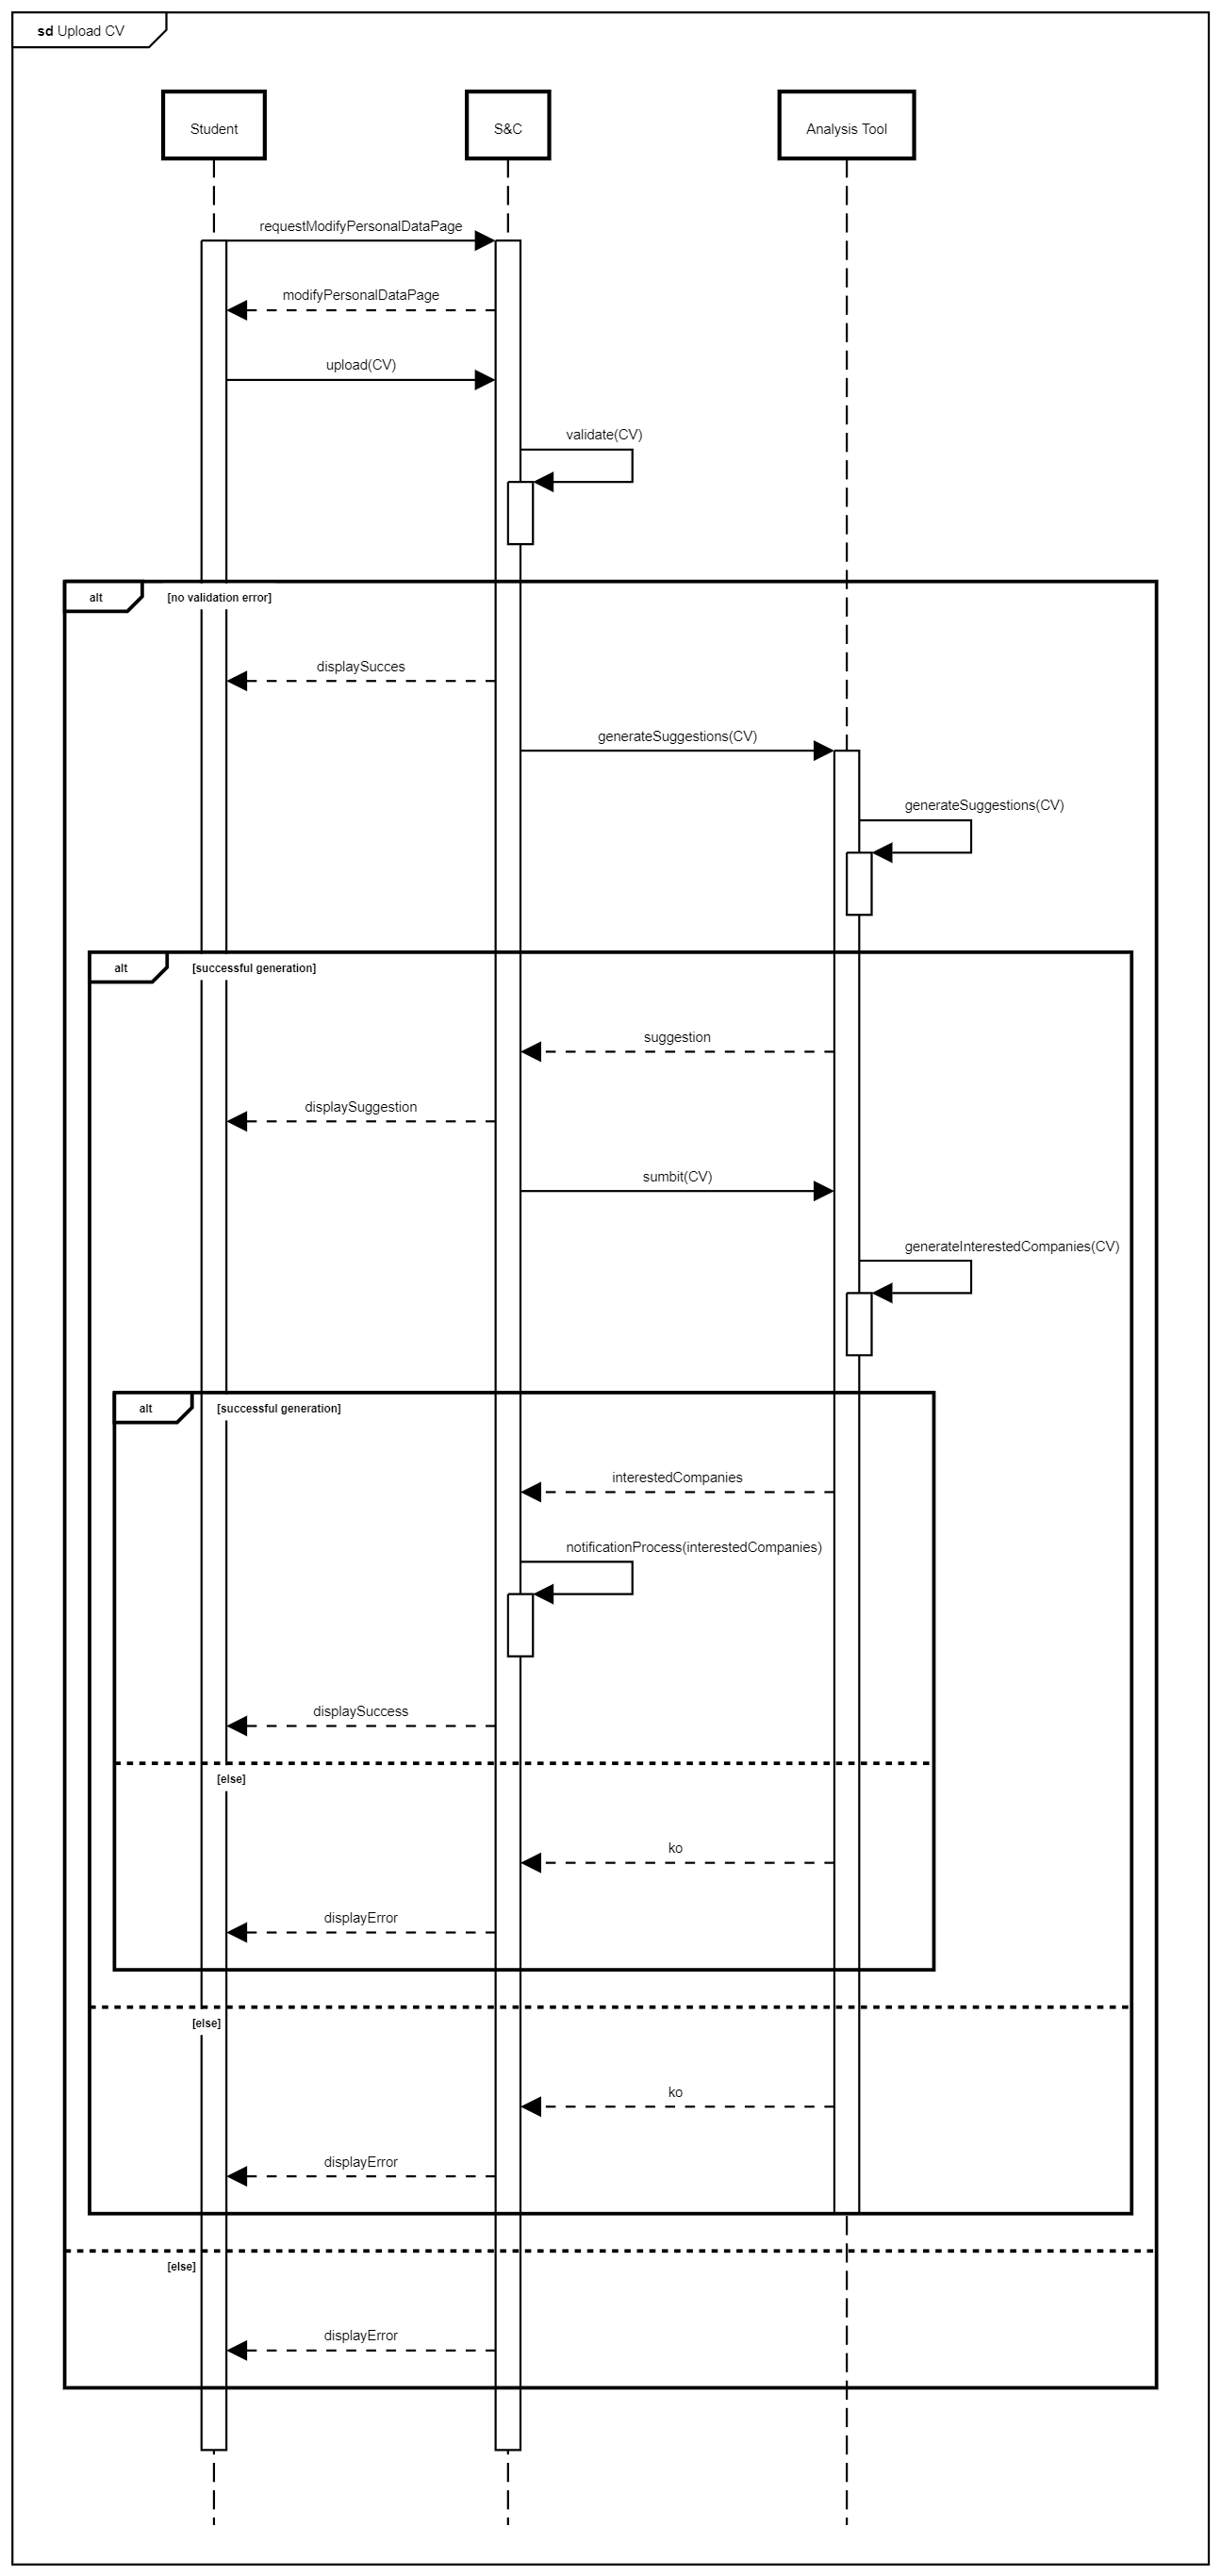
\includegraphics[width=0.8\textwidth]{Images/sd/UploadCV}
    \caption{Upload CV - Sequence Diagram}
    \label{fig:SDuploadCV}
\end{figure}


\begin{center}
    \begin{longtable}{|p{2.5cm}|p{10cm}|}
        \hline
        \rowcolor[HTML]{5C8A99}
        \textbf{Use Case \cuc} & \textbf{View available internships} \\ \hline
        \textbf{Entry \newline conditions} & The Student is in the view available internships section of S\&C and wants to see available internships.\\ \hline
        \textbf{Actor} & Student \\ \hline
        \textbf{Event flow} &
        \begin{enumerate}
            \item The Student clicks on the `View internships` button.
            \item The System shows the list, that includes basic information for each internship such as the company and the position.
        \end{enumerate}
        \\ \hline
        \textbf{Exit \newline condition} & The Student successfully views the available internships. \\ \hline
        \textbf{Exception} &
        \begin{itemize}
            \item If an error occurs while the visualizing the available internships the System displays an error.
        \end{itemize}
        \\ \hline
    \end{longtable}
\end{center}

\begin{figure}[H]
    \centering
    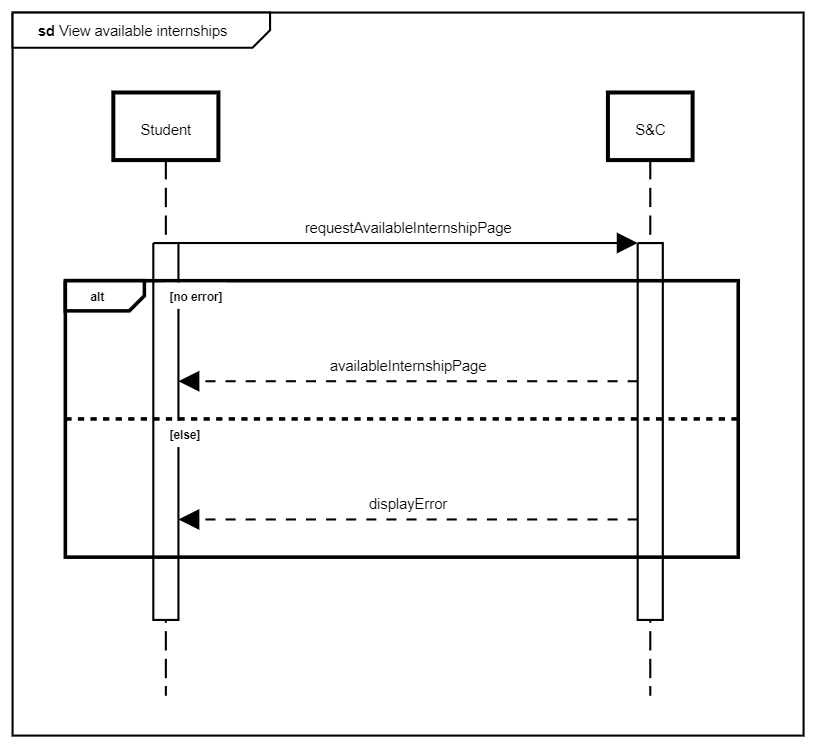
\includegraphics[width=0.8\textwidth]{Images/sd/ViewAvailableInternships}
    \caption{View available intenrships - Sequence Diagram}
    \label{fig:SDviewavint}
\end{figure}


\begin{center}
    \begin{longtable}{|p{2.5cm}|p{10cm}|}
        \hline
        \rowcolor[HTML]{5C8A99}
        \textbf{Use Case \cuc} & \textbf{View recommended internships} \\ \hline
        \textbf{Actor} & Student, Analysis Tool \\ \hline
        \textbf{Entry \newline conditions} & The Student is in the view available internships section of S\&C and wants to see recommended internships.\\ \hline
        \textbf{Event flow - Main} &
        \begin{enumerate}
            \item The Student clicks on the `recommended` button.
            \item The Analysis Tool compute the recommended internship based on Student information.
            \item The System redirects the Student to the view recommended section.
        \end{enumerate}
        \\ \hline
        \textbf{Event flow - Optional} &
        \begin{enumerate}
            \item The Student select an internship from the list to view its details.
            \item The Student filter by name the recommended internships by writing in the appropriate search box.
        \end{enumerate}
        \\ \hline
        \textbf{Exit \newline condition} & The Student successfully views the recommended internships. \\ \hline
        \textbf{Exception} &
        \begin{itemize}
            \item If an error occurs while redirecting the Student the System displays an error.
            \item If the are no recommended internships the System displays an error.
            \item If an error occurs while showing the details of an internship the System displays an error.
            \item If an error occurs while filtering recommended internships the System displays an error.
            \item If an error occurs while the Analysis tool compute the recommendations the System displays an error.
        \end{itemize}
        \\ \hline
    \end{longtable}
\end{center}

\begin{figure}[H]
    \centering
    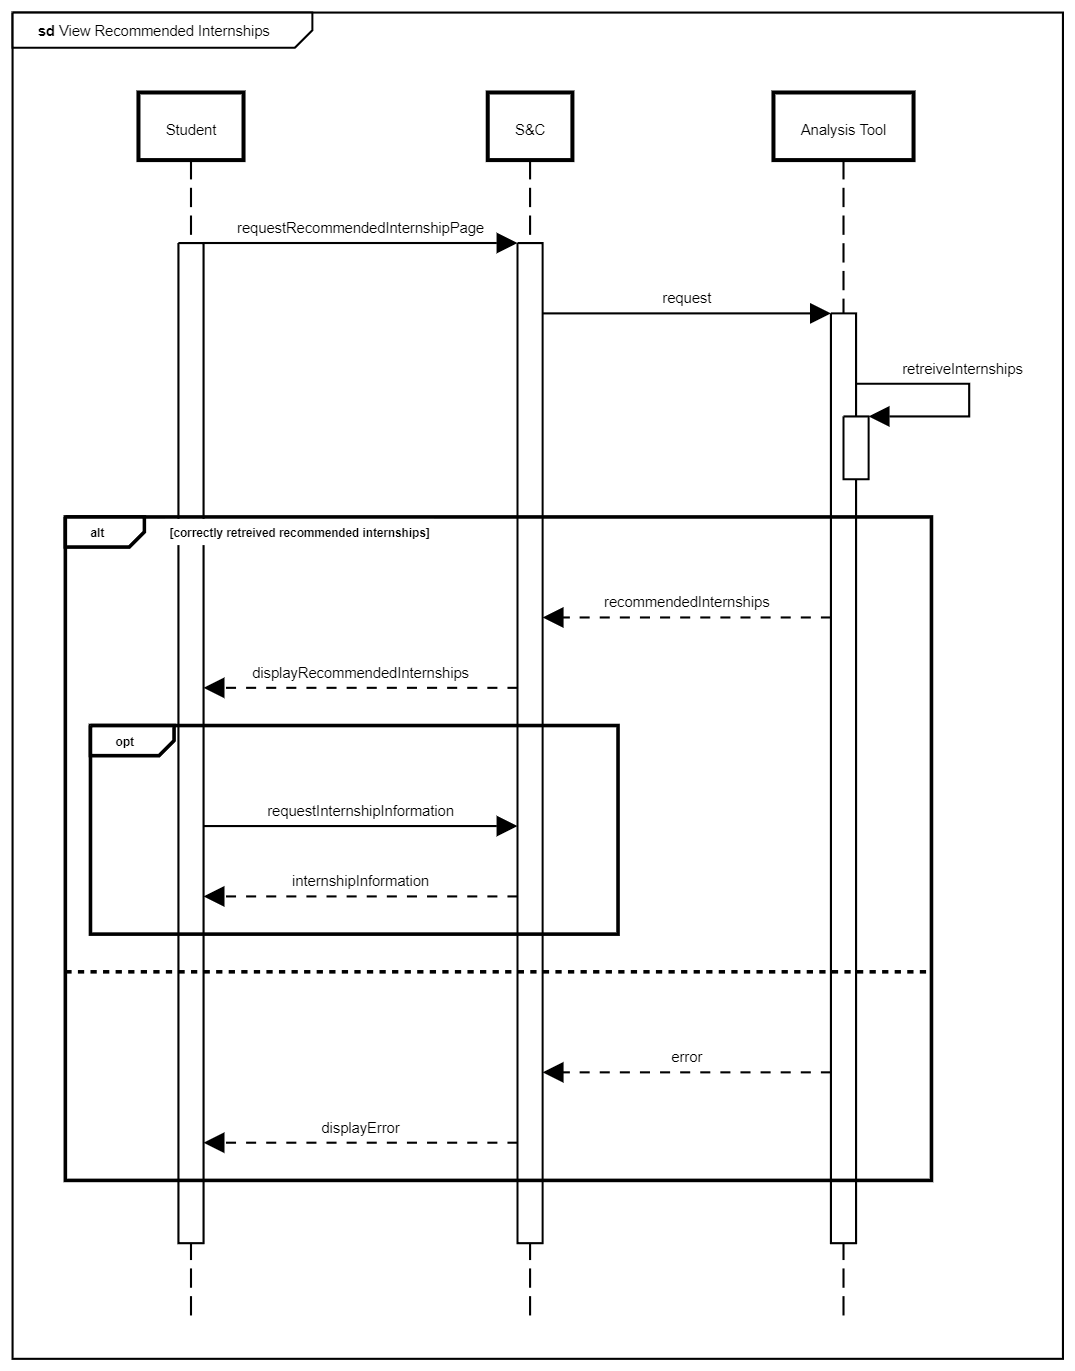
\includegraphics[width=0.8\textwidth]{Images/sd/ViewRecommendedInternships}
    \caption{View recommended intenrships - Sequence Diagram}
    \label{fig:SDviewRecInt}
\end{figure}

\begin{center}
    \begin{longtable}{|p{2.5cm}|p{10cm}|}
        \hline
        \rowcolor[HTML]{5C8A99}
        \textbf{Use Case \cuc} & \textbf{Search for internships } \\ \hline
        \textbf{Actor} & Student \\ \hline
        \textbf{Entry \newline conditions} & The Student is in the view available internships section of S\&C and wants to search for internships.\\ \hline
        \textbf{Event flow - Main} &
        \begin{enumerate}
            \item The Student clicks on the search bar.
            \item The Student insert the name of a company or the position for which he wants to search.
            \item The System displays the filtered results.
        \end{enumerate}
        \\ \hline
        \textbf{Event flow - Optional} &
        \begin{enumerate}
            \item The Student select an internship from the list to view its details.
        \end{enumerate}
        \\ \hline
        \textbf{Exit \newline condition} & The Student successfully searched for internships. \\ \hline
        \textbf{Exception} &
        \begin{itemize}
            \item If the are no matching internships the System displays an error.
        \end{itemize}
        \\ \hline
    \end{longtable}
\end{center}

\begin{figure}[H]
    \centering
    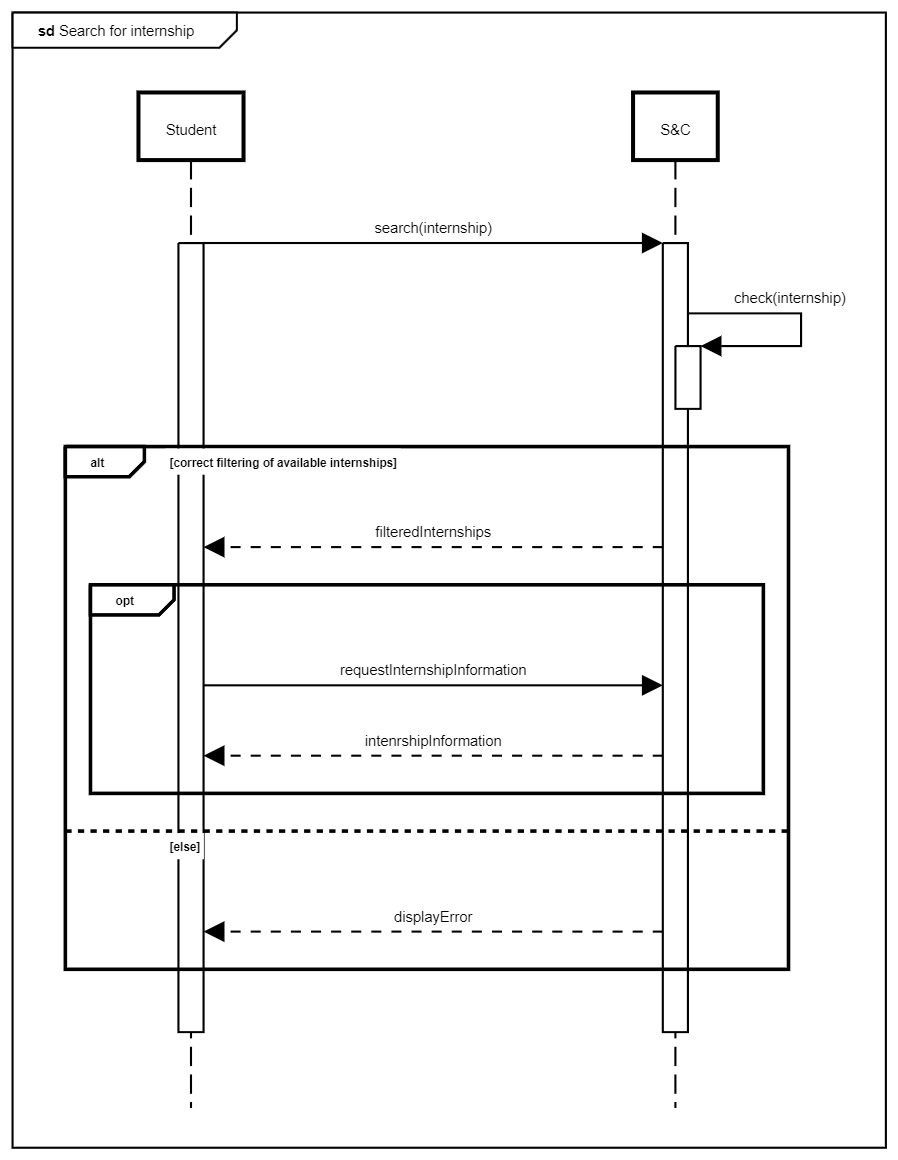
\includegraphics[width=0.8\textwidth]{Images/sd/SearchForInternship}
    \caption{Search for intenrships - Sequence Diagram}
    \label{fig:SDsearchint}
\end{figure}

\begin{center}
    \begin{longtable}{|p{2.5cm}|p{10cm}|}
        \hline
        \rowcolor[HTML]{5C8A99}
        \textbf{Use Case \cuc} & \textbf{Apply for internship} \\ \hline
        \textbf{Actor} & Student \\ \hline
        \textbf{Entry \newline conditions} & The Student selected an internship and wants to apply for the position. \\ \hline
        \textbf{Event flow} &
        \begin{enumerate}
            \item The Student navigate to the detail page of the internship.
            \item The Student click on the `apply` button.
            \item The System sends a notification to the Company for the interview.
        \end{enumerate}
        \\ \hline
        \textbf{Exit \newline condition} & The Student successfully applied for an interview on the platform. \\ \hline
        \textbf{Exception} &
        \begin{itemize}
            \item If an error occurs while validating the information the System displays an error.
            \item If an error occurs while sending a notification the System displays an error.
        \end{itemize}
        \\ \hline
    \end{longtable}
\end{center}

\begin{figure}[H]
    \centering
    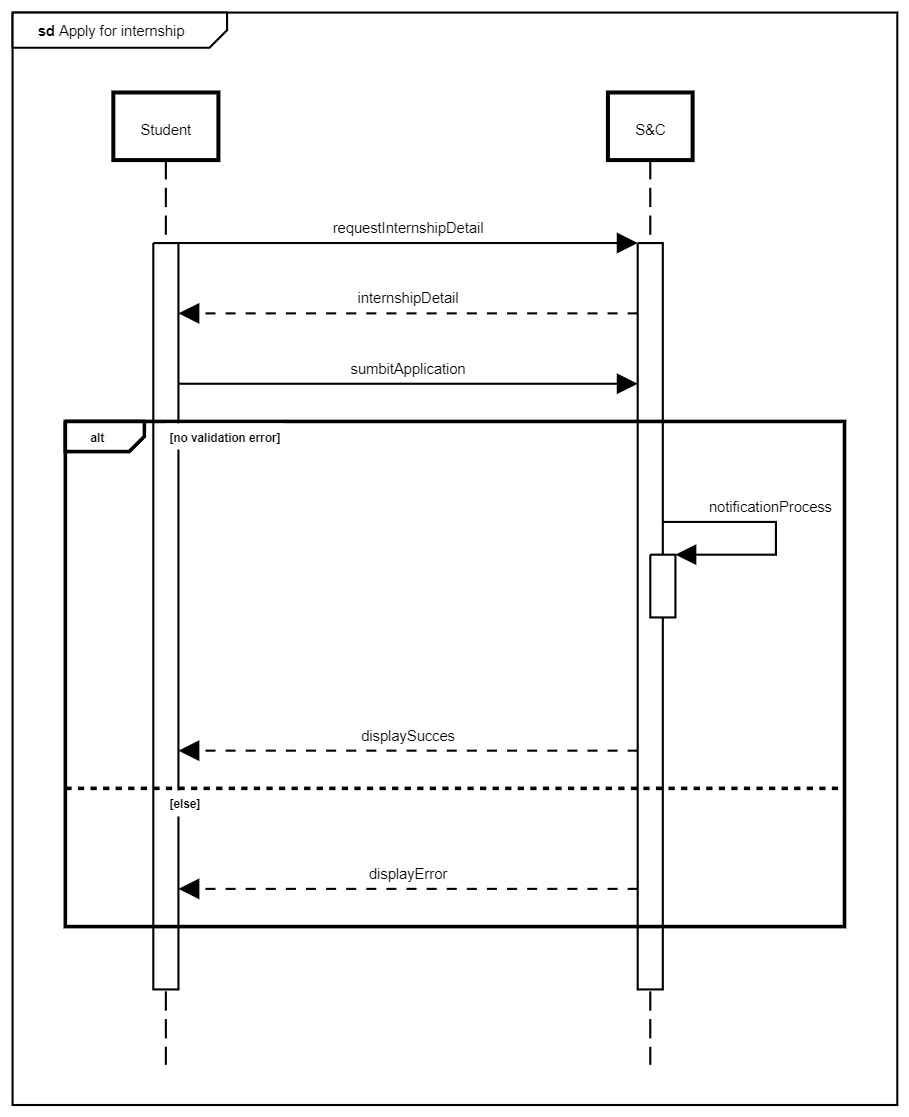
\includegraphics[width=0.8\textwidth]{Images/sd/ApplyForInternship}
    \caption{Apply for intenrships - Sequence Diagram}
    \label{fig:SDapply}
\end{figure}

\begin{center}
    \begin{longtable}{|p{2.5cm}|p{10cm}|}
        \hline
        \rowcolor[HTML]{5C8A99}
        \textbf{Use Case \cuc} & \textbf{Fill structured questioner} \\ \hline
        \textbf{Actor} & Student \\ \hline
        \textbf{Entry \newline conditions} & The Student is in the fill structured questioner section of the S\&C platform and wants to complete the questioner for the interview.\\ \hline
        \textbf{Event flow} &
        \begin{enumerate}
            \item The Student fills the form with the responses to the questions.
            \item The Student clicks on the `submit` button.
            \item The System validates the information and saves the responses of the questioner.
        \end{enumerate}
        \\ \hline
        \textbf{Exit \newline condition} & The Student successfully filled and submitted the structured questioner.  \\ \hline
        \textbf{Exception} &
        \begin{itemize}
            \item If there are missing obligatory fields then the System displays an error.
            \item If an error occurs while validating and saving the information the System displays an error.
        \end{itemize}
        \\ \hline
    \end{longtable}
\end{center}

\begin{figure}[H]
    \centering
    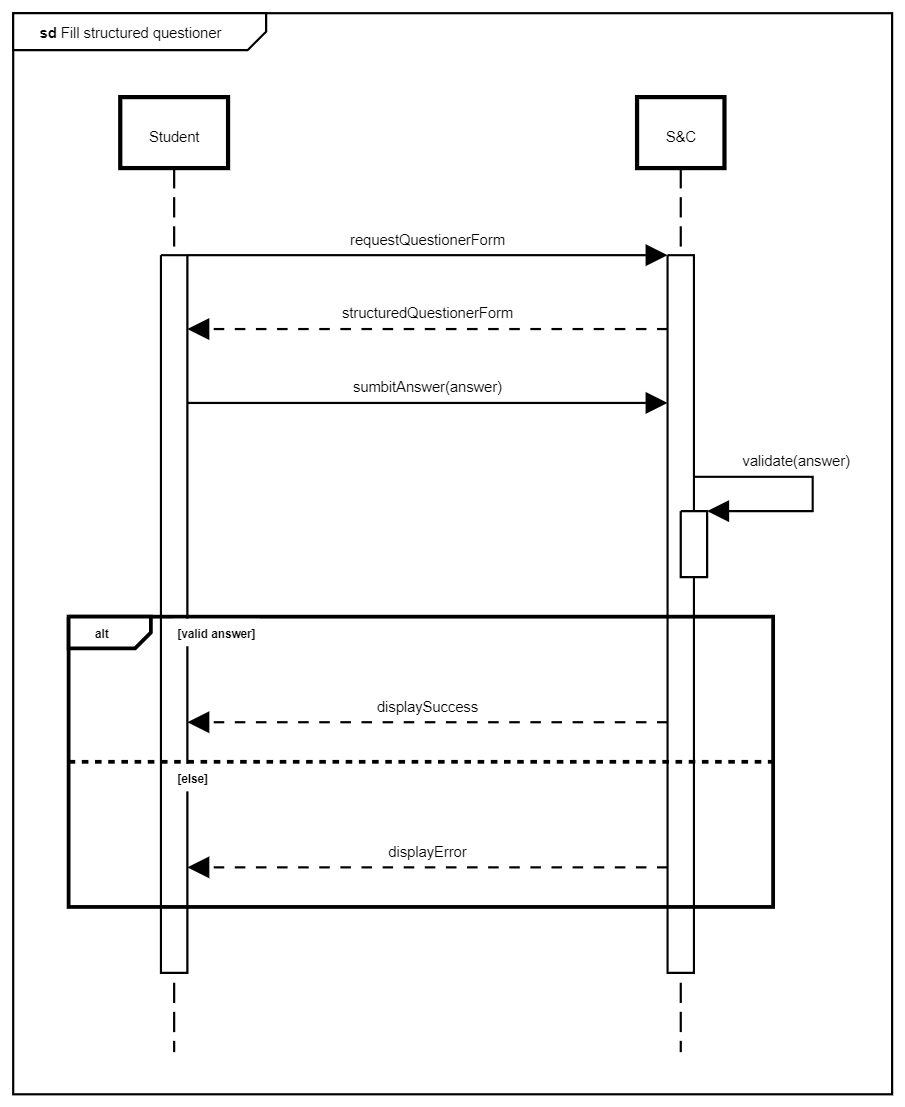
\includegraphics[width=0.8\textwidth]{Images/sd/FillStructuredQuestioner}
    \caption{Fill structured questioner - Sequence Diagram}
    \label{fig:SDfillquestioner}
\end{figure}

\begin{center}
    \begin{longtable}{|p{2.5cm}|p{10cm}|}
        \hline
        \rowcolor[HTML]{5C8A99}
        \textbf{Use Case \cuc} & \textbf{View complaints} \\ \hline
        \textbf{Actor} & University \\ \hline
        \textbf{Entry \newline conditions} & The University is in the view complaints of S\&C and wants to view complaints for a specific internship.\\ \hline
        \textbf{Event flow - Main} &
        \begin{enumerate}
            \item The University clicks on the internship it wants to see the detail of.
            \item The System displays the received complaints for that internship.
        \end{enumerate}
        \\ \hline
        \textbf{Event flow - Optional} &
        \begin{enumerate}
            \item The University fill the response section.
            \item The University clicks on the `send` button.
            \item The System notifies the correct recipient with the message notification.
        \end{enumerate}
        \\ \hline
        \textbf{Exit \newline condition} & The University successfully viewed the complaints, and if wanted, sent a response. \\ \hline
        \textbf{Exception} &
        \begin{itemize}
            \item If the are no complaints the System displays a `no complaints` message.
            \item If an error occurs while sending a notification the System displays an error.
            \item If the response is empty while being sent the System displays an error.
        \end{itemize}
        \\ \hline
    \end{longtable}
\end{center}

\begin{figure}[H]
    \centering
    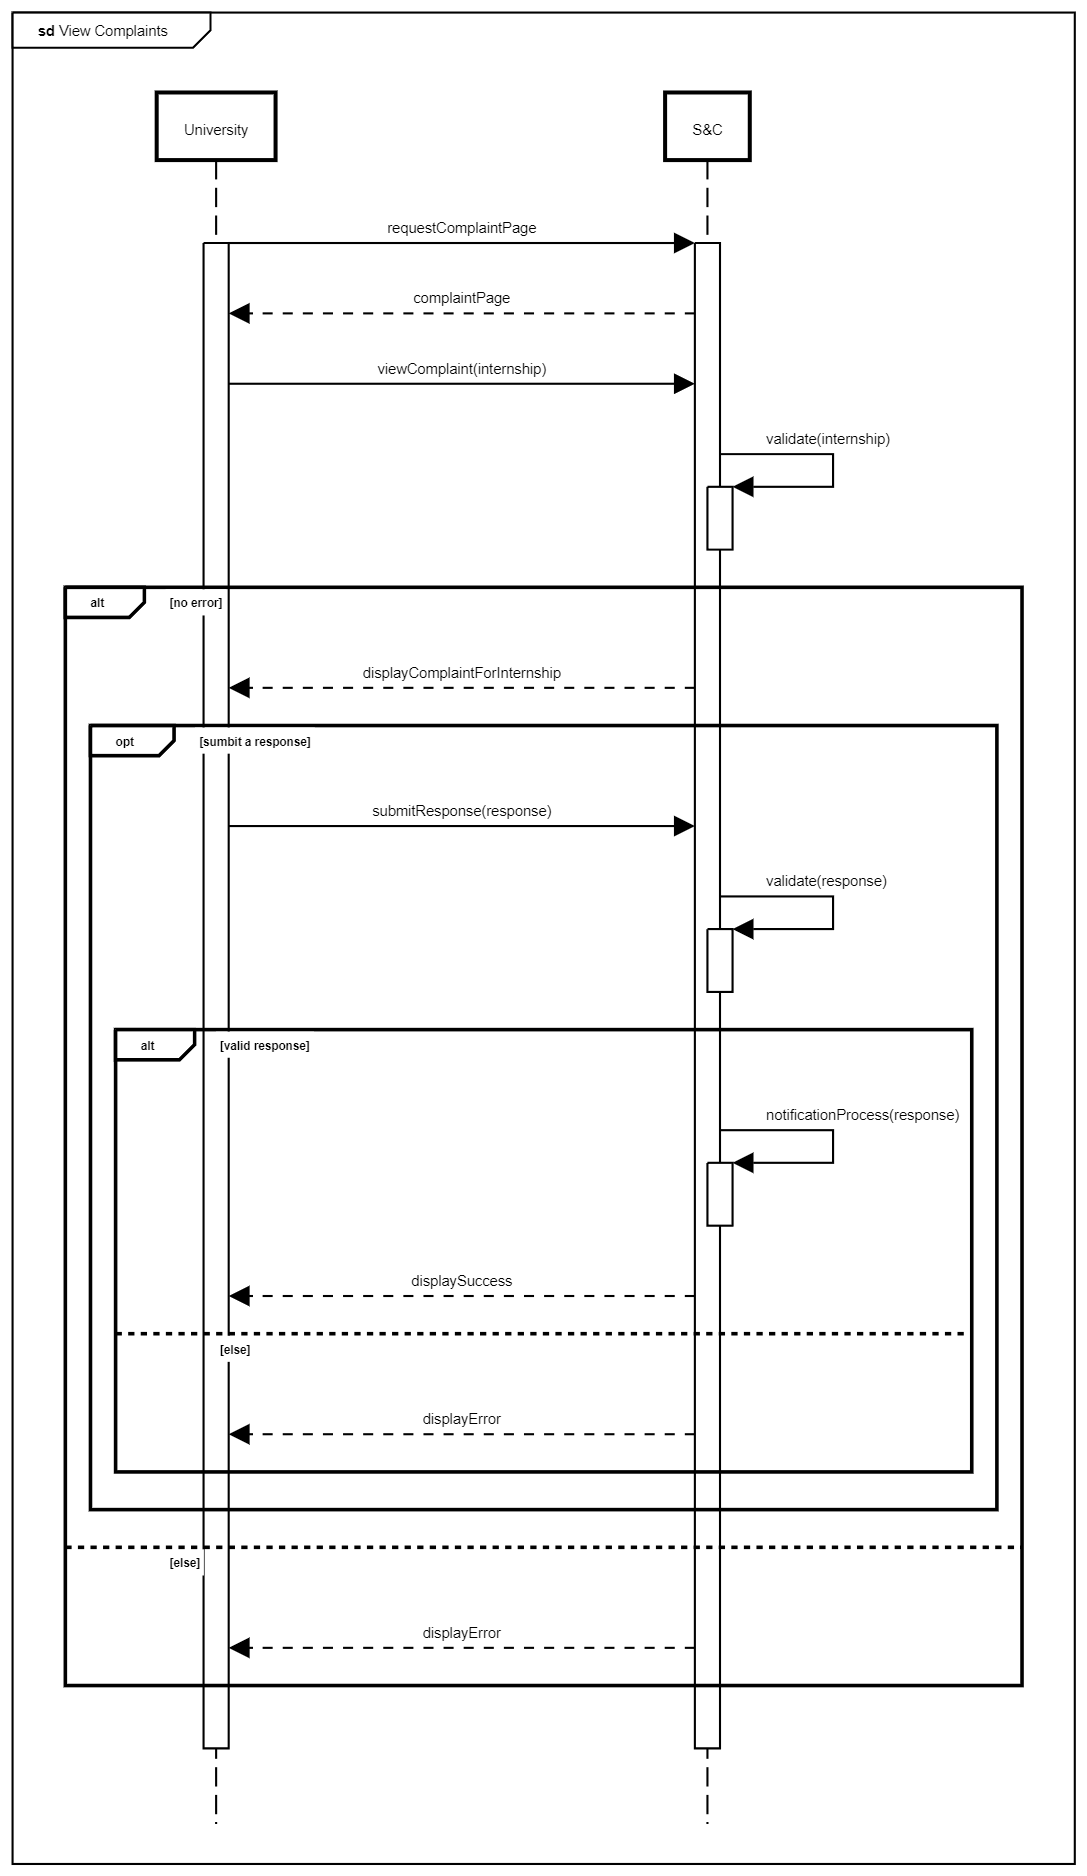
\includegraphics[width=0.8\textwidth]{Images/sd/ViewComplaints}
    \caption{View complaints - Sequence Diagram}
    \label{fig:SDviewcompl}
\end{figure}

\begin{center}
    \begin{longtable}{|p{2.5cm}|p{10cm}|}
        \hline
        \rowcolor[HTML]{5C8A99}
        \textbf{Use Case \cuc} & \textbf{Terminate internships} \\ \hline
        \textbf{Actor} & University\\ \hline
        \textbf{Entry \newline conditions} & The University is in the manage internships section of S\&C and wants to terminate a specific internship.\\ \hline
        \textbf{Event flow} &
        \begin{enumerate}
            \item The University clicks on the internship it wants to manage.
            \item The System displays the termination form for that internship.
            \item The University fills the form with the reason of termination.
            \item The University clicks on the `terminate` button.
            \item The System validates the information and terminate the internship.
            \item The System notifies the parties of the internship with a message notification.
        \end{enumerate}
        \\ \hline
        \textbf{Exit \newline condition} & The University successfully terminated the internship. \\ \hline
        \textbf{Exception} &
        \begin{itemize}
            \item If the are no internships to manage the System displays a `no internship to manage` message.
            \item If an error occurs while sending a notification the System displays an error.
            \item If the reason of termination is empty while being sent the System displays an error.
            \item If an error occurs while validating and terminating the internship the System displays and error.
            \item If an error occurs while showing the the termination form for an internship the System displays an error.
        \end{itemize}
        \\ \hline
    \end{longtable}
\end{center}

\begin{figure}[H]
    \centering
    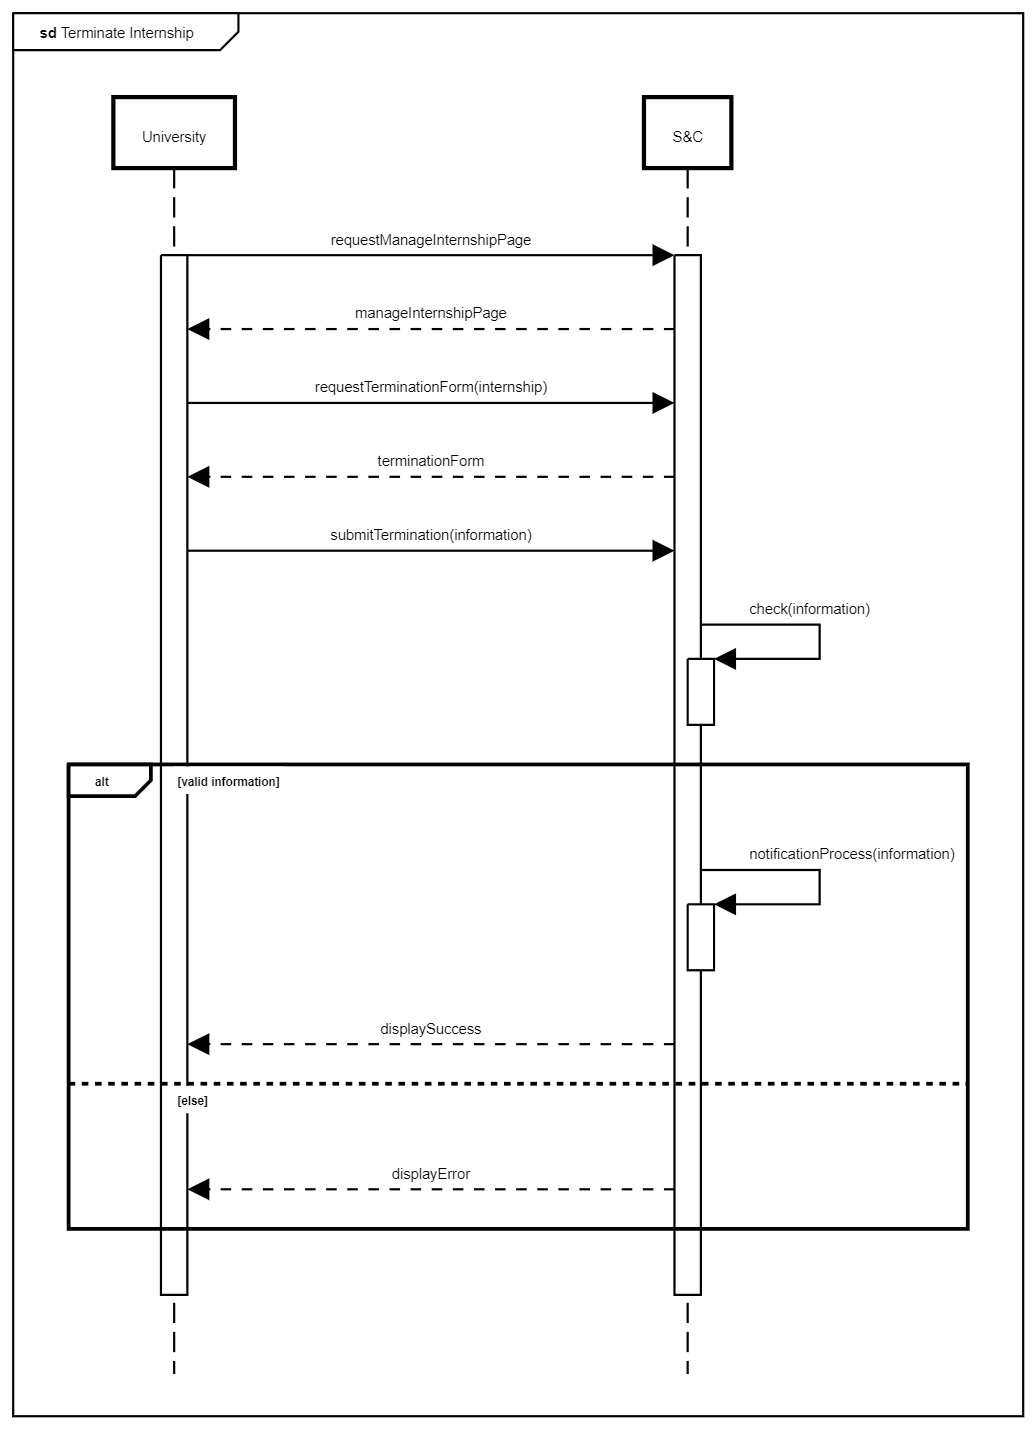
\includegraphics[width=0.8\textwidth]{Images/sd/TerminateInternship}
    \caption{Terminate internship - Sequence Diagram}
    \label{fig:SDterminate}
\end{figure}





\subsection{Mapping on requirements}\label{subsec:mapping-on-requirements}
\setcounter{uc}{1}
\setcounter{req}{1}

\begin{center}
    \begin{tabular}{|c|c|c|}
        \hline
        \rowcolor[HTML]{5C8A99}
        \textbf{Use Case} & \textbf{Requirement} \\ \hline
        \rowcolor[HTML]{FFFFFF} % Bianco
        UC1 & R1 \\ \hline
        \rowcolor[HTML]{F0F0F0} % Grigio chiaro
        UC2 & R2 \\ \hline
        \rowcolor[HTML]{FFFFFF} % Bianco
        UC3 & R21, R5, R15\\ \hline
        \rowcolor[HTML]{F0F0F0} % Grigio chiaro
        UC4 & R7 \\ \hline
        \rowcolor[HTML]{FFFFFF} % Bianco
        UC5 & R8\\ \hline
        \rowcolor[HTML]{F0F0F0} % Grigio chiaro
        UC6 & R9\\ \hline
        \rowcolor[HTML]{FFFFFF} % Bianco
        UC7 & R10\\ \hline
        \rowcolor[HTML]{F0F0F0} % Grigio chiaro
        UC8 & R11, R13 \\ \hline
        \rowcolor[HTML]{FFFFFF} % Bianco
        UC9 & R14\\ \hline
        \rowcolor[HTML]{F0F0F0} % Grigio chiaro
        UC10 & R17\\ \hline
        \rowcolor[HTML]{FFFFFF} % Bianco
        UC11 & R22\\ \hline
        \rowcolor[HTML]{F0F0F0} % Grigio chiaro
        UC12 & R8\\ \hline
        \rowcolor[HTML]{FFFFFF} % Bianco
        UC13 & R3, R6, R16 \\ \hline
        \rowcolor[HTML]{F0F0F0} % Grigio chiaro
        UC14 & R4 \\ \hline
        \rowcolor[HTML]{FFFFFF} % Bianco
        UC15 & R7 \\ \hline
        \rowcolor[HTML]{F0F0F0} % Grigio chiaro
        UC16 & R20\\ \hline
        \rowcolor[HTML]{FFFFFF} % Bianco
        UC17 & R8\\ \hline
        \rowcolor[HTML]{F0F0F0} % Grigio chiaro
        UC18 & R12\\ \hline
        \rowcolor[HTML]{FFFFFF} % Bianco
        UC19 & R18\\ \hline
        \rowcolor[HTML]{F0F0F0} % Grigio chiaro
        UC20 & R19\\ \hline
    \end{tabular}
\end{center}

\setcounter{g}{1}

\begin{center}
    \begin{longtable}{|l|p{13.5cm}|}
        \hline
        \rowcolor[HTML]{5C8A99}
        \textbf{ID} & \textbf{Description} \\ \hline
        \rowcolor[HTML]{E7E0FA} % Goal color
        G1 & Allow students and companies to provide information (internships, CVs) \\ \hline
        \rowcolor[HTML]{FFF9C4} % Domain color
        D1 & The internet connection works properly. \\ \hline
        \rowcolor[HTML]{FFF9C4} % Domain color
        D2 & User* have a suitable working device \\ \hline
        \rowcolor[HTML]{FFF9C4} % Domain color
        D3 & Students are enrolled in a subscribed university \\ \hline
        \rowcolor[HTML]{FFF9C4} % Domain color
        D4 & Universities, students, and companies receive information sent from the system \\ \hline
        \hline\rowcolor[HTML]{FFDAB9} % Blue poli
        R1 & The system allows the User* to sign up if it’s not already registered \\ \hline
        \hline\rowcolor[HTML]{FFDAB9} % Blue poli
        R2 & The system allows the User* to log if it’s already registered \\ \hline
        \hline\rowcolor[HTML]{FFDAB9} % Blue poli
        R3 & The system allows logged students to upload their CVs \\ \hline
        \hline\rowcolor[HTML]{FFDAB9} % Blue poli
        R21 & The system allows companies to publish internships. \\ \hline
    \end{longtable}
\end{center}

\begin{center}
    \begin{longtable}{|l|p{13.5cm}|}
        \hline
        \rowcolor[HTML]{5C8A99}
        \textbf{ID} & \textbf{Description} \\ \hline
        \rowcolor[HTML]{E7E0FA} % Goal color
        G2 & Allow companies to advertise internships \\ \hline
        \rowcolor[HTML]{FFF9C4} % Domain color
        D1 & The internet connection works properly \\ \hline
        \rowcolor[HTML]{FFF9C4} % Domain color
        D2 & User* have a suitable working device \\ \hline
        \rowcolor[HTML]{FFF9C4} % Domain color
        D4 & Universities, students, and companies receive information sent from the system \\ \hline
        \hline\rowcolor[HTML]{FFDAB9} % Blue poli
        R21 & Allow companies to create and manage internships \\ \hline
    \end{longtable}
\end{center}

\begin{center}
    \begin{longtable}{|l|p{13.5cm}|}
        \hline
        \rowcolor[HTML]{5C8A99}
        \textbf{ID} & \textbf{Description} \\ \hline
        \rowcolor[HTML]{E7E0FA} % Goal color
        G3 & Allow students to search for internships \\ \hline
        \rowcolor[HTML]{FFF9C4} % Domain color
        D1 & The internet connection works properly \\ \hline
        \rowcolor[HTML]{FFF9C4} % Domain color
        D2 & User* have a suitable working device \\ \hline
        \rowcolor[HTML]{FFF9C4} % Domain color
        D3 & Students are enrolled in a subscribed university \\ \hline
        \rowcolor[HTML]{FFF9C4} % Domain color
        D4 & Universities, students, and companies receive information sent from the system \\ \hline
        \hline\rowcolor[HTML]{FFDAB9} % Blue poli
        R20 & The system allows Students to proactively search for internships. \\ \hline
    \end{longtable}
\end{center}

\begin{center}
    \begin{longtable}{|l|p{13.5cm}|}
        \hline
        \rowcolor[HTML]{5C8A99}
        \textbf{ID} & \textbf{Description} \\ \hline
        \rowcolor[HTML]{E7E0FA} % Goal color
        G4 & Allow students and companies to deal with the recommendation process \\ \hline
        \rowcolor[HTML]{FFF9C4} % Domain color
        D1 & The internet connection works properly. \\ \hline
        \rowcolor[HTML]{FFF9C4} % Domain color
        D2 & User* have a suitable working device \\ \hline
        \rowcolor[HTML]{FFF9C4} % Domain color
        D3 & Students are enrolled in a subscribed university \\ \hline
        \rowcolor[HTML]{FFF9C4} % Domain color
        D4 & Universities, students, and companies receive information sent from the system \\ \hline
        \hline\rowcolor[HTML]{FFDAB9} % Blue poli
        R5 & The system allows students to be informed about internships they are suitable for \\ \hline
        \hline\rowcolor[HTML]{FFDAB9} % Blue poli
        R6 &The system allows companies to be informed about the availability of students’ CVs corresponding to their need \\ \hline
        \hline\rowcolor[HTML]{FFDAB9} % Blue poli
        R7 & The system allow companies and students to view a suitable recommendation \\ \hline
        \hline\rowcolor[HTML]{FFDAB9} % Blue poli
        R8 & The system allows companies and students to establish a contact after finding a suitable recommendation \\ \hline
    \end{longtable}
\end{center}

\begin{center}
    \begin{longtable}{|l|p{13.5cm}|}
        \hline
        \rowcolor[HTML]{5C8A99}
        \textbf{ID} & \textbf{Description} \\ \hline
        \rowcolor[HTML]{E7E0FA} % Goal color
        G5 & Allow the management of interview and selections \\ \hline
        \rowcolor[HTML]{FFF9C4} % Domain color
        D1 & The internet connection works properly. \\ \hline
        \rowcolor[HTML]{FFF9C4} % Domain color
        D2 & User* have a suitable working device \\ \hline
        \rowcolor[HTML]{FFF9C4} % Domain color
        D3 & Students are enrolled in a subscribed university \\ \hline
        \rowcolor[HTML]{FFF9C4} % Domain color
        D4 & Universities, students, and companies receive information sent from the system \\ \hline
        \rowcolor[HTML]{FFF9C4} % Domain color
        D5 & Students and companies are responsible for conducting interviews independently \\ \hline
        \hline\rowcolor[HTML]{FFDAB9} % Blue poli
        R9 & The system allows companies to set up interview (information/question) \\ \hline
        \hline\rowcolor[HTML]{FFDAB9} % Blue poli
        R10 & The system allows companies to conduct interviews \\ \hline
        \hline\rowcolor[HTML]{FFDAB9} % Blue poli
        R11 & The system allows companies to view answer from structured questionnaires \\ \hline
        \hline\rowcolor[HTML]{FFDAB9} % Blue poli
        R12 & The system allows students to compile structured questionnaires \\ \hline
        \hline\rowcolor[HTML]{FFDAB9} % Blue poli
        R13 &The system allows companies to finalize the selections \\ \hline
        \hline\rowcolor[HTML]{FFDAB9} % Blue poli
        R22 & The system allows Users to view planned interviews. \\ \hline
    \end{longtable}
\end{center}

\begin{center}
    \begin{longtable}{|l|p{13.5cm}|}
        \hline
        \rowcolor[HTML]{5C8A99}
        \textbf{ID} & \textbf{Description} \\ \hline
        \rowcolor[HTML]{E7E0FA} % Goal color
        G6 & Allow the Analysis Tool to collect various kinds of information regarding the internships \\ \hline
        \rowcolor[HTML]{FFF9C4} % Domain color
        D1 & The internet connection works properly \\ \hline
        \rowcolor[HTML]{FFF9C4} % Domain color
        D2 & User* have a suitable working device \\ \hline
        \rowcolor[HTML]{FFF9C4} % Domain color
        D4 & Universities, students, and companies receive information sent from the system \\ \hline
        \hline\rowcolor[HTML]{FFDAB9} % Blue poli
        R14 & The system allows the User to provide feedback and suggestions to feed the Analysis Tool \\ \hline
    \end{longtable}
\end{center}

\begin{center}
    \begin{longtable}{|l|p{13.5cm}|}
        \hline
        \rowcolor[HTML]{5C8A99}
        \textbf{ID} & \textbf{Description} \\ \hline
        \rowcolor[HTML]{E7E0FA} % Goal color
        G7 & Allow suggestions to students and companies regarding how to make submissions \\ \hline
        \rowcolor[HTML]{FFF9C4} % Domain color
        D1 & The internet connection works properly \\ \hline
        \rowcolor[HTML]{FFF9C4} % Domain color
        D2 & User* have a suitable working device \\ \hline
        \rowcolor[HTML]{FFF9C4} % Domain color
        D4 & Universities, students, and companies receive information sent from the system \\ \hline
        \hline\rowcolor[HTML]{FFDAB9} % Blue poli
        R15 &The system allow companies to retrieve suggestions regarding internships’ descriptions \\ \hline
        \hline\rowcolor[HTML]{FFDAB9} % Blue poli
        R16 & The system provides suggestions regarding CVs for students \\ \hline
    \end{longtable}
\end{center}

\begin{center}
    \begin{longtable}{|l|p{13.5cm}|}
        \hline
        \rowcolor[HTML]{5C8A99}
        \textbf{ID} & \textbf{Description} \\ \hline
        \rowcolor[HTML]{E7E0FA} % Goal color
        G8 & Allow students and companies to establish a contact \\ \hline
        \rowcolor[HTML]{FFF9C4} % Domain color
        D1 & The internet connection works properly \\ \hline
        \rowcolor[HTML]{FFF9C4} % Domain color
        D2 & User* have a suitable working device \\ \hline
        \rowcolor[HTML]{FFF9C4} % Domain color
        D3 & Students are enrolled in a subscribed university \\ \hline
        \rowcolor[HTML]{FFF9C4} % Domain color
        D4 & Universities, students, and companies receive information sent from the system \\ \hline
        \hline\rowcolor[HTML]{FFDAB9} % Blue poli
        R8 & The system allows companies and students to establish a contact after finding a suitable recommendation \\ \hline
    \end{longtable}
\end{center}
% TODO : it is the same goal ? ...
\begin{center}
    \begin{longtable}{|l|p{13.5cm}|}
        \hline
        \rowcolor[HTML]{5C8A99}
        \textbf{ID} & \textbf{Description} \\ \hline
        \rowcolor[HTML]{E7E0FA} % Goal color
        G9 & Allow students and companies to perform the selection process \\ \hline
        \rowcolor[HTML]{FFF9C4} % Domain color
        D1 & The internet connection works properly \\ \hline
        \rowcolor[HTML]{FFF9C4} % Domain color
        D2 & User* have a suitable working device \\ \hline
        \rowcolor[HTML]{FFF9C4} % Domain color
        D3 & Students are enrolled in a subscribed university \\ \hline
        \rowcolor[HTML]{FFF9C4} % Domain color
        D4 & Universities, students, and companies receive information sent from the system \\ \hline
        \rowcolor[HTML]{FFF9C4} % Domain color
        D5 & Students and companies are responsible for conducting interviews independently \\ \hline
        \hline\rowcolor[HTML]{FFDAB9} % Blue poli
        R13 & Manage selection process \\ \hline
    \end{longtable}
\end{center}

\begin{center}
    \begin{longtable}{|l|p{13.5cm}|}
        \hline
        \rowcolor[HTML]{5C8A99}
        \textbf{ID} & \textbf{Description} \\ \hline
        \rowcolor[HTML]{E7E0FA} % Goal color
        G10 & Allow students and companies to provide feedbacks \\ \hline
        \rowcolor[HTML]{FFF9C4} % Domain color
        D1 & The internet connection works properly. \\ \hline
        \rowcolor[HTML]{FFF9C4} % Domain color
        D2 & User* have a suitable working device \\ \hline
        \rowcolor[HTML]{FFF9C4} % Domain color
        D3 & Students are enrolled in a subscribed university \\ \hline
        \rowcolor[HTML]{FFF9C4} % Domain color
        D4 & Universities, students, and companies receive information sent from the system \\ \hline
        \hline\rowcolor[HTML]{FFDAB9} % Blue poli
        R17 & The system allows the User to complain and communicate problems through provided spaces \\ \hline
    \end{longtable}
\end{center}

\begin{center}
    \begin{longtable}{|l|p{13.5cm}|}
        \hline
        \rowcolor[HTML]{5C8A99}
        \textbf{ID} & \textbf{Description} \\ \hline
        \rowcolor[HTML]{E7E0FA} % Goal color
        G11 & Allow universities to monitor internships (complaints) \\ \hline
        \rowcolor[HTML]{FFF9C4} % Domain color
        D1 & The internet connection works properly. \\ \hline
        \rowcolor[HTML]{FFF9C4} % Domain color
        D2 & User* have a suitable working device \\ \hline
        \rowcolor[HTML]{FFF9C4} % Domain color
        D3 & Students are enrolled in a subscribed university \\ \hline
        \rowcolor[HTML]{FFF9C4} % Domain color
        D4 & Universities, students, and companies receive information sent from the system \\ \hline
        \hline\rowcolor[HTML]{FFDAB9} % Blue poli
        R18 & The system allows universities to view complaints about internships of their students \\ \hline
        \hline\rowcolor[HTML]{FFDAB9} % Blue poli
        R19 & The system allows universities to terminate internships of their students \\ \hline
    \end{longtable}
\end{center}
% ---------------------------------------------------------------------------------------------------------------------- %

\section{Performance requirements}\label{sec:performance-requirements}
\subsection{Number of users}\label{subsec:number-of-users}
Research data from UNESCO suggests that around $254$ million students are enrolled in universities around the world.
Assuming that $15\%$ are potentially searching for an internship, we would like to at least attract $10\%$ of that number, so the system needs to handle roughly $4$ million students.
We also need to consider the number of companies, increasing the number of potential user up $4.5$ million.
Moreover, the amount of universities is negligible compared the previous estimates, thus the platform need to be able to handle at least $4$ to $5$ million of users.
\subsection{Data storage}\label{subsec:data-storage}
The system needs to manage information of students, companies and universities, such as access credentials and personal information.
Among the possible data that needs to be stored, we can also find the CVs of students, scheduled interviews, internships information and so on.
There is also the need to save data fed to the Analysis Tool, as well as all the complains, messages and notifications that are exchanged on the platform.
\subsection{Time response}\label{subsec:time-response}
To guarantee a satisfactory user experience the system should handle requests in the domain of milliseconds in critical activities while in non critical sections the system should tolerate up to seconds in terms of time response.
% ---------------------------------------------------------------------------------------------------------------------- %

\section{Design constraints}\label{sec:design-constraints}
\subsection{Standards compliance}\label{subsec:standards-compliance}
The system must comply with data protection regulations of the countries it will operate in, for example it needs to respect the European Union's General Data Protection Regulation (GDPR).
Another important respected standard is the ISO/IEC 27001, fundamental for risk management, cyber-resilience and operational excellence.
\subsection{Hardware limitations}\label{subsec:hardware-limitations}
The systems can be use from any device with a compatible web browser and an internet connection.
\subsection{Any other constraint}\label{subsec:any-other-constraint}
There are no other constraints.

% ---------------------------------------------------------------------------------------------------------------------- %

\section{Software system attributes}\label{sec:software-system-attributes}
\subsection{Reliability}\label{subsec:reliability}
The system will need to run for long periods of time, so it needs to be reliable.
To achieve reliability a coding standard must be defined, that is a set of guidelines and best practices that will need to be followed during the development of the system.
Additionally replication can be used to further ensure reliability.
\subsection{Availability}\label{subsec:availability}
The system will need to be ready to be used whenever a user desires, so it needs to be available.
The goal would be to achieve $99.9\%$ availability, and this can be done by utilizing replication.
\subsection{Security}\label{subsec:security}
% TODO: access rights?
The system will store personal information of students, as well as information on companies and universities.
That's why it must ensure data privacy through encryption of local data, when the information is stored.
Regarding information exchanged over the internet thanks to HTTPS will be able to guarantee an encrypted communication.
\subsection{Maintainability}\label{subsec:maintainability}
The system must be designed and implemented with the goal for maintainability, taking in consideration also scalability.
\subsection{Portability}\label{subsec:portability}
The system is a web application and can run on basically any web browser and internet connection capable device.
For this reason the only portability requirement would be a dynamic user interface that can be correctly visualized on most type of standard screen resolution.